\newpage
\section{HAI ĐƯỜNG THẲNG SONG SONG}
\subsection{LÝ THUYẾT CẦN NHỚ}
\subsubsection{Vị trí tương đối của hai đường thẳng trong không gian}
\begin{dn}
	Cho hai đường thẳng $a$ và $b$ trong không gian. Khi đó có thể xảy ra một trong hai trường hợp sau:
	\begin{enumerate}[\bf TH 1.]
		\item Có một mặt phẳng chứa $a$ và $b$. Khi đó ta nói $a$ và $b$ đồng phẳng. Theo kết quả của hình học phẳng, có ba khả năng sau đây xảy ra:
		\begin{itemize}
			\item Nếu $a$ và $b$ có hai điểm chung thì ta nói $a$ trùng $b$, kí hiệu $a \equiv b$.
			\item Nếu $a$ và $b$ có một điểm chung duy nhất $M$ thì ta nói $a$ và $b$ cắt nhau tại $M$, kí hiệu $a \cap b = M$.
			\item Nếu $a$ và $b$ không có điểm chung thì ta nói $a$ và $b$ song song với nhau, kí hiệu $a \parallel b$.
		\end{itemize}
		\begin{tabular}{C{0.3\linewidth}C{0.3\linewidth}C{0.3\linewidth}}
			\begin{tikzpicture}[font=\footnotesize, line join=round, line cap=round, >=stealth, scale=1]
				\path (0,0) coordinate (p)+(3,0) coordinate (q) (70:2) coordinate (s)+(3,0) coordinate (r)
				pic[draw, angle radius=5mm, "$\alpha$"]{angle=q--p--s};
				\draw (p)--(q)--(r)--(s)--cycle
				(0.5,0.5)--(3,1.5)node[above]{$a$}node[below]{$b$};
				\node[below] at (current bounding box.south) {$a\equiv b$};
			\end{tikzpicture}
	&
			\begin{tikzpicture}[font=\footnotesize, line join=round, line cap=round, >=stealth, scale=1]
				\path (0,0) coordinate (p)+(3,0) coordinate (q) (70:2) coordinate (s)+(3,0) coordinate (r)
				pic[draw, angle radius=5mm, "$\alpha$"]{angle=q--p--s};
				\draw (p)--(q)--(r)--(s)--cycle
				(0.5,0.5)--(3,1.5)node[above]{$a$}
				(1,1.3)--(3,0.5)node[above]{$b$};
				\fill (1.75,1) circle (1pt)node[above]{$M$};
				\node[below] at (current bounding box.south) {$a\cap b=M$};
			\end{tikzpicture}
	&
			\begin{tikzpicture}[font=\footnotesize, line join=round, line cap=round, >=stealth, scale=1]
				\path (0,0) coordinate (p)+(3,0) coordinate (q) (70:2) coordinate (s)+(3,0) coordinate (r)
				pic[draw, angle radius=5mm, "$\alpha$"]{angle=q--p--s};
				\draw (p)--(q)--(r)--(s)--cycle
				(0.5,0.25)--++(10:2.5)node[above]{$a$}
				(0.5,1)--++(10:2.25)node[above]{$b$};
				\node[below] at (current bounding box.south) {$a\parallel b$};
			\end{tikzpicture}
		\end{tabular}
		\item Không có mặt phẳng nào chứa cả $a$ và $b$. Khi đó ta nói hai đường thẳng $a$ và $b$ chéo nhau hay $a$ chéo với $b$.
	\end{enumerate}
	\begin{center}
		\begin{tikzpicture}[font=\footnotesize, line join=round, line cap=round, >=stealth, scale=1]
			\path (0,0) coordinate (p)+(3,0) coordinate (q) (70:2) coordinate (s)+(3,0) coordinate (r)
			pic[draw, angle radius=5mm, "$\alpha$"]{angle=q--p--s};
			\draw (p)--(q)--(r)--(s)--cycle
			(0.5,0.25)--++(10:2.5)node[above]{$a$}
			(2,1)--(2,2.5)node[right]{$b$} (2,0)--(2,-0.5);
			\draw[dashed] (2,1)--(2,0);
			\fill (2,1) circle (1pt)node[above right]{$I$};
			\node[below] at (current bounding box.south) {$a$, $b$ chéo nhau};
		\end{tikzpicture}
	\end{center}
\end{dn}

\begin{dn}
	Hai đường thẳng gọi là \textbf{song song} nếu chúng nằm trong cùng một mặt phẳng và không có điểm chung.
\end{dn}

\begin{note}
	\begin{enumerate}
		\item Hai đường thẳng gọi là \textbf{chéo nhau} nếu chúng không đồng phẳng.
		\item Cho hai đường thẳng song song $a$ và $b$. Có duy nhất một mặt phẳng chứa hai đường thẳng đó, kí hiệu mp$(a,b)$.
	\end{enumerate}
\end{note}

\subsubsection{Tính chất cơ bản về hai đường thẳng song song}
\begin{dl}
	Trong không gian, qua một điểm nằm ngoài một đường thẳng, có một và chỉ một đường thẳng song song với đường thẳng đó.
	\begin{center}
		\begin{tikzpicture}[font=\footnotesize, line join=round, line cap=round, >=stealth, scale=1]
			\path (0,0) coordinate (p)+(3,0) coordinate (q) (70:2) coordinate (s)+(3,0) coordinate (r)
			pic[draw, angle radius=5mm, "$\alpha$"]{angle=q--p--s};
			\draw (p)--(q)--(r)--(s)--cycle
			(0.5,0.25)--++(10:2.5)node[above]{$a$}
			(0.5,0.75)--++(10:2.25)node[above]{$b$};
			\fill ($(0.5,0.75)+(10:1)$) circle (1pt)node[above]{$M$};
		\end{tikzpicture}
	\end{center}
\end{dl}

\begin{dl}
	(\textit{Định lý về giao tuyến của ba mặt phẳng}) Nếu ba mặt phẳng đôi một cắt nhau theo ba giao tuyến phân biệt thì ba giao tuyến ấy hoặc đồng quy hoặc đôi một song song.
	\begin{center}
		\begin{tabular}{C{0.5\linewidth}C{0.5\linewidth}}
			\begin{tikzpicture}[font=\footnotesize]
				\path (0,0) coordinate (A) (0,2.5) coordinate (B)
				(A)++(-20:1.5) coordinate (ap) (B)++(-20:1.5) coordinate (bp)
				(A)++(-170:1.5) coordinate (at) (B)++(-170:1.5) coordinate (bt)
				pic[draw, angle radius=5mm, "$P$"]{angle=at--bt--B}
				pic[draw, angle radius=5mm, "$Q$"]{angle=B--bp--ap}
				(0,2) coordinate (C) (A)++(-20:1) coordinate (c1) (A)++(-170:1.25) coordinate (c2)
				pic[draw, angle radius=5mm, "$R$"]{angle=c1--c2--C};
				\draw (C)--(B)--(bp)--(ap)--(c1) (C)--(B)--(bt)--(at)--(c2) (c2)--(C)node[pos=0.5,left]{$a$}--(c1)node[pos=0.5,right]{$b$}--cycle;
				\draw[dashed] (C)--(A)node[pos=0.7,left]{$c$} (c1)--(A)--(c2);
				\fill (C) circle (1pt)node[left]{$I$};
			\end{tikzpicture}
	&
			\begin{tikzpicture}[font=\footnotesize]
				\path (0,0) coordinate (A) (0,2.5) coordinate (B)
				(A)++(-20:1.5) coordinate (ap) (B)++(-20:1.5) coordinate (bp)
				(A)++(-170:1.5) coordinate (at) (B)++(-170:1.5) coordinate (bt)
				pic[draw, angle radius=5mm, "$P$"]{angle=at--bt--B}
				pic[draw, angle radius=5mm, "$Q$"]{angle=B--bp--ap}
				(0,2) coordinate (C) (A)++(-20:0.75) coordinate (c1)+(0,2.5) coordinate (c1t) (A)++(-170:0.75) coordinate (c2)+(0,2.5) coordinate (c2t)
				pic[draw, angle radius=5mm, "$R$"]{angle=c1--c2--c2t};
				\draw (0,2.3)--(B)--(bp)--(ap)--(c1) (B)--(bt)--(at)--(c2) (c1)--(c1t)node[pos=0.5,right]{$b$}--(c2t)--(c2)node[pos=0.5,left]{$a$}--cycle;
				\draw[dashed] (A)--++(0,2.3)node[pos=0.5,left]{$c$} (c1)--(A)--(c2);
			\end{tikzpicture}
		\end{tabular}
	\end{center}
\end{dl}

\begin{hq}
	Nếu hai mặt phẳng phân biệt lần đường đi qua hai đường thẳng song song thì giao tuyến của chúng (nếu có) song song với hai đường thẳng đó hoặc trùng với một trong hai đường thẳng đó.
	\begin{center}
		\begin{tabular}{C{0.3\linewidth}C{0.3\linewidth}C{0.3\linewidth}}
			\begin{tikzpicture}[font=\footnotesize, line join=round, line cap=round, >=stealth, scale=1]
				\path
				(0,0) coordinate (a)+(-150:1.5)coordinate(at)+(-20:1.5)coordinate(ap)
				(0,2.5) coordinate (b)+(-150:1.5)coordinate(bt)+(-20:1.5)coordinate(bp)
				pic[draw, angle radius=4mm, "$\alpha$"]{angle=at--bt--b}
				pic[draw, angle radius=4mm, "$\beta$"]{angle=b--bp--ap};
				\draw (a)--(at)--(bt)--(b)--cycle
				(a)--(ap)--(bp)--(b);
				\draw (0,1)node[right]{$d$}
				(-0.5,0)--++(0,2)node[left, midway]{$d_1$}
				(0.7,0)--++(0,2)node[right, midway]{$d_2$};
				\node[below] at (current bounding box.south) {$d\parallel d_1$, $d\parallel d_2$};
			\end{tikzpicture}
	&
			\begin{tikzpicture}[font=\footnotesize, line join=round, line cap=round, >=stealth, scale=1]
				\path
				(0,0) coordinate (a)+(-150:1.5)coordinate(at)+(-20:1.5)coordinate(ap)
				(0,2.5) coordinate (b)+(-150:1.5)coordinate(bt)+(-20:1.5)coordinate(bp)
				pic[draw, angle radius=4mm, "$\alpha$"]{angle=at--bt--b}
				pic[draw, angle radius=4mm, "$\beta$"]{angle=b--bp--ap};
				\draw (a)--(at)--(bt)--(b)--cycle
				(a)--(ap)--(bp)--(b);
				\draw (0,1)node[right]{$d$}node[left]{$d_1$}
				% (-0.5,0)--++(0,2)node[left, midway]{$d_1$}
				(0.7,0)--++(0,2)node[right, midway]{$d_2$};
				\node[below] at (current bounding box.south) {$d\equiv d_1$, $d\parallel d_2$};
			\end{tikzpicture}
	&
			\begin{tikzpicture}[font=\footnotesize, line join=round, line cap=round, >=stealth, scale=1]
				\path
				(0,0) coordinate (a)+(-150:1.5)coordinate(at)+(-20:1.5)coordinate(ap)
				(0,2.5) coordinate (b)+(-150:1.5)coordinate(bt)+(-20:1.5)coordinate(bp)
				pic[draw, angle radius=4mm, "$\alpha$"]{angle=at--bt--b}
				pic[draw, angle radius=4mm, "$\beta$"]{angle=b--bp--ap};
				\draw (a)--(at)--(bt)--(b)--cycle
				(a)--(ap)--(bp)--(b);
				\draw (0,1)node[left]{$d$}node[right]{$d_2$}
				(-0.5,0)--++(0,2)node[left, midway]{$d_1$};
				% (0.7,0)--++(0,2)node[right, midway]{$d_2$};
				\node[below] at (current bounding box.south) {$d\parallel d_1$, $d\equiv d_2$};
			\end{tikzpicture}
		\end{tabular}
	\end{center}
\end{hq}

\begin{dl}
	Hai đường thẳng phân biệt cùng song với một đường thẳng thứ ba thì song song với nhau.
\end{dl}

\begin{note}
	Khi hai đường thẳng phân biệt $a$, $b$ cùng song song với đương thẳng $c$ thì ta có thể kí hiệu $a\parallel b \parallel c$ và gọi là {\it ba đường thẳng song song}.
\end{note}

\subsection{PHÂN LOẠI VÀ PHƯƠNG PHÁP GIẢI TOÁN}
\begin{dang}{Xét vị trí tương đối của hai đường thẳng trong không gian}
	Dựa theo lý thuyết từ\indam{Định nghĩa 2.1} và\indam{Định ngĩa 2.2}.
\end{dang}

\begin{vd}
	Cho hình chóp $S.ABCD$ có đáy $ABCD$ là hình bình hành. Xét vị trí tương đối của mỗi cặp đường thẳng sau
	\begin{multicols}{3}
		\begin{enumerate}
			\item $AC$ và $BD$;
			\item $AB$ và $CD$;
			\item $SA$ và $BD$.
		\end{enumerate}
	\end{multicols}
\loigiai{
	\immini
	{\begin{enumerate}
		\item Ta có $AC$ cắt $BD$.
		\item Do $ABCD$ là hình bình hành nên $AB\parallel CD$.
		\item Ta có $SA$ và $BD$ chéo nhau.
	\end{enumerate}}
	{\begin{tikzpicture}[font=\footnotesize, line join=round, line cap=round, >=stealth, scale=1]
		\path (0,0) coordinate (A) (-150:1.5) coordinate (B) (3,0) coordinate (D) ($(B)+(3,0)$) coordinate (C) (1,2) coordinate (S);
		\draw (S)--(B)--(C)--(D)--cycle (S)--(C);
		\draw[dashed] (B)--(A)--(D) (S)--(A);
		\foreach \x/\g in {S/90, A/135, B/-135, C/-45, D/45}{\fill (\x) circle (1pt)+(\g:0.3)node{$\x$};}
	\end{tikzpicture}}
	}
\end{vd}

\begin{vd}
	Cho tứ diện $ABCD$ có $M$, $N$ lần lượt là trung điểm của $AB$ và $AC$. Xét vị trí tương đối của mỗi cặp đường thẳng sau
	\begin{multicols}{3}
		\begin{enumerate}
			\item $AN$ và $CD$;
			\item $MN$ và $BC$;
			\item $BD$ và $AC$.
		\end{enumerate}
	\end{multicols}
\loigiai{
	\immini
	{\begin{enumerate}
		\item Ta có $AN$ cắt $CD$ tại $C$.
		\item Xét $\triangle ABC$ có $MN$ là đường trung bình. Suy ra $MN\parallel BC$.
		\item Ta có $BD$ và $AC$ chéo nhau.
	\end{enumerate}}
	{\begin{tikzpicture}[font=\footnotesize, line join=round, line cap=round, >=stealth, scale=1]
		\path (0,0) coordinate (B) (-25:3) coordinate (C) (4,0) coordinate (D) (1,3) coordinate (A)
		($(A)!1/2!(B)$) coordinate (M)
		($(A)!1/2!(C)$) coordinate (N);
		\draw (A)--(B)--(C)--(D)--cycle (A)--(C) (M)--(N);
		\draw[dashed] (B)--(D);
		\foreach \x/\g in {A/90, B/135, C/-90, D/45, M/180, N/45}{\fill (\x) circle (1pt)+(\g:0.3)node{$\x$};}
	\end{tikzpicture}}
	}
\end{vd}

\begin{vd}
	Cho tứ diện $ABCD$. Lấy $M$, $P$ là hai điểm phân biệt trên cạnh $AB$ (khác $A$ và $B$); $N$, $Q$ là hai điểm phân biệt trên cạnh $CD$ (khác $C$ và $D$). Xét vị trí tương đối của hai đường thẳng $MN$ và $PQ$.
\loigiai{
	\immini
	{Ta chứng minh hai đường thẳng $MN$ và $PQ$ chéo nhau.\\
			Giả sử hai đường thẳng $MN$ và $PQ$ không chéo nhau, tức là chúng đồng phẳng. Gọi $(\alpha)$ là mặt phẳng chứa cả hai đường thẳng này.\\			
			Vì $M, P \in AB$ và $M \ne P$, nên $AB \subset (\alpha)$.	\\		
			Tương tự, $N, Q \in CD$ và $N \ne Q$, nên $CD \subset (\alpha)$.	\\		
			Suy ra hai cạnh $AB$ và $CD$ cùng nằm trên mặt phẳng $(\alpha)$.	Điều này mâu thuẫn với giả thiết $AB$ và $CD$ là hai cạnh đối của tứ diện $ABCD$, nên không thể đồng phẳng.	\\		
			Vậy hai đường thẳng $MN$ và $PQ$ textbf{chéo nhau}.	
	}
	{\begin{tikzpicture}[font=\footnotesize, line join=round, line cap=round, >=stealth, scale=1]
		\path (0,0) coordinate (B) (3,0) coordinate (D) (-40:2) coordinate (C) (1,2) coordinate (A)
		($(A)!1/3!(B)$) coordinate (M) ($(A)!2/3!(B)$) coordinate (P) ($(C)!1/4!(D)$) coordinate (N) ($(C)!3/4!(D)$) coordinate (Q);
		\draw (A)--(B)--(C)--(D)--cycle (A)--(C);
		\draw[dashed] (B)--(D) (M)--(N)--(P)--(Q);
		\foreach \x/\g in {A/90, B/180, D/0, C/-90, M/135, N/-45, Q/-45, P/135}{\fill (\x) circle (1pt)+(\g:0.3)node{$\x$};}
	\end{tikzpicture}}
	}
\end{vd}

\begin{dang}{Chứng minh hai đường thẳng song song}
	Áp dụng phối hợp bằng các kiến thức:
	\begin{enumerate}[\bf 1.]
		\item Thông qua hình học phẳng. Áp dụng tính chất của đường trung bình trong tam giác, hình thang; định lý Thalès đảo, \ldots
		\item Áp dụng\indam{Định lí 2.2},\indam{Định lí 2.3}.
	\end{enumerate}
\end{dang}

\begin{vd}[\textit{Trích SBT Toán Chân trời sáng tạo}]
	Cho hình chóp $S.ABCD$ có đáy $ABCD$ là hình bình hành. Gọi $I$, $J$ lần lượt là trung điểm của các cạnh $SA$ và $SB$. Chứng minh rằng $IJ \parallel AB$, từ đó suy ra $IJ \parallel CD$.
	\loigiai{
	\immini
	{Vì $I$, $J$ lần lượt là trung điểm của các đoạn thẳng $SA$, $SB$ nên $IJ$ là đường trung bình của tam giác $SAB$.\\
	Do đó, $IJ \parallel AB$.\\
	Mà $ABCD$ là hình bình hành nên $AB \parallel CD$.\\
	Vậy $IJ \parallel CD$ (vì cùng song song với đường thẳng $AB$).}
	{\begin{tikzpicture}[font=\footnotesize, line join=round, line cap=round, >=stealth, scale=1]
	\path (0,0) coordinate (A) (-150:1.5) coordinate (B) (3,0) coordinate (D) ($(B)+(3,0)$) coordinate (C) (1,2) coordinate (S)
	($(S)!1/2!(A)$) coordinate (I) ($(S)!1/2!(B)$) coordinate (J);
	\draw (S)--(B)--(C)--(D)--cycle (S)--(C);
	\draw[dashed] (B)--(A)--(D) (S)--(A) (I)--(J);
	\foreach \x/\g in {S/90, A/135, B/-135, C/-45, D/45, I/0, J/180}{\fill (\x) circle (1pt)+(\g:0.3)node{$\x$};}
	\end{tikzpicture}}
	}
\end{vd}

\begin{vd}[\textit{Trích SBT Toán Cánh Diều}]
	Cho tứ diện $ABCD$. Gọi $G_1$, $G_2$ lần lượt là trọng tâm của các tam giác $ABC$ và $ABD$. Chứng minh hai đường thẳng $G_1G_2$ và $CD$ song song với nhau.
	\loigiai{
	\immini
	{Gọi $M$, $N$ lần lượt là trung điểm của $BC$, $BD$. Khi đó\\
	Xét $\triangle ABC$ ta có $\dfrac{AG_1}{AM} = \dfrac{2}{3}$.\\
	Xét $\triangle ABD$ ta có $\dfrac{AG_2}{AN} = \dfrac{2}{3}$.\\
	Suy ra trong $\triangle ANM$ có $\dfrac{AG_1}{AM} = \dfrac{AG_2}{AN} = \dfrac{2}{3}$.\\
	Theo định lý Thalès đảo, suy ra $G_1G_2 \parallel MN$.\\
	Mặt khác $MN$ là đường trung bình của tam giác $BCD$ nên $MN \parallel CD$.\\
	Vậy $G_1G_2 \parallel CD$.}
	{\begin{tikzpicture}[font=\footnotesize, line join=round, line cap=round, >=stealth, scale=1]
	\path (0,0) coordinate (B) (-50:2) coordinate (C) (4,0) coordinate (D) (1,3) coordinate (A)
	($(B)!1/2!(C)$) coordinate (M) ($(B)!1/2!(D)$) coordinate (N)
	($(A)!2/3!(M)$) coordinate (G_1) ($(A)!2/3!(N)$) coordinate (G_2);
	\draw (A)--(B)--(C)--(D)--cycle (A)--(C) (A)--(M);
	\draw[dashed] (B)--(D) (G_1)--(G_2) (M)--(N)--(A);
	\foreach \x/\g in {A/90, B/135, C/-90, D/45, M/180, N/45, G_1/180, G_2/30}{\fill (\x) circle (1pt)+(\g:0.3)node{$\x$};}
	\end{tikzpicture}}
	}
\end{vd}

\begin{vd}[\textit{Trích SBT Toán Kết nối tri thức}]
Cho tứ diện $ABCD$. Gọi $E$, $F$ lần lượt là trung điểm của các cạnh $AB$, $AC$ và $M$ là một điểm bất kì thuộc cạnh $AD$. Giả sử $ME$ cắt $BD$ tại $N$ và $MF$ cắt $CD$ tại $P$. Chứng minh rằng $NP \parallel EF$.
\loigiai{
	\immini
	{Xét ba mặt phẳng $(MEF)$, $(BCD)$ và $(ABC)$, ta có
	\begin{itemize}
		\item $(MEF) \cap (BCD) = NP$;
		\item $(MEF) \cap (ABC) = EF$;
		\item $(BCD) \cap (ABC) = BC$.
	\end{itemize}
	Theo\indam{Định lý 2.2}, ba giao tuyến này hoặc đồng quy, hoặc đôi một song song.\\
	Vì $EF$ là đường trung bình của tam giác $ABC$ nên $EF$ song song với $BC$.\\
	Do đó ba giao tuyến $NP$, $EF$, $BC$ đôi một song song.\\
	Hay $NP\parallel EF$.}
	{\begin{tikzpicture}[font=\footnotesize, line join=round, line cap=round, >=stealth, scale=1]
	\path (0,0) coordinate (D) (-30:2) coordinate (C) (4,0) coordinate (B) (1,3) coordinate (A)
	($(A)!1/2!(B)$) coordinate (E) ($(A)!1/2!(C)$) coordinate (F)
	($(A)!1/4!(D)$) coordinate (M)
	(intersection of M--E and B--D) coordinate (N)
	(intersection of M--F and C--D) coordinate (P);
	\draw (A)--(D)--(P)--(N)--(E)--(A) (A)--(C) (M)--(P) (E)--(F);
	\draw[dashed] (D)--(B)--(C) (M)--(E)--(B)--(N);
	\foreach \x/\g in {A/90, B/45, C/-90, D/135, M/180, N/0, P/-90, E/45, F/180}{\fill (\x) circle (1pt)+(\g:0.3)node{$\x$};}
	\end{tikzpicture}}
	}
\end{vd}

\begin{dang}{Xác định giao tuyến của hai mặt phẳng chứa hai đường thẳng song song}
	Áp dụng\indam{Hệ quả 2.1}.
\end{dang}

\begin{vd}[\textit{Trích SBT Toán Chân trời sáng tạo}]
	Cho hình chóp $S.ABCD$ có đáy $ABCD$ là hình bình hành. Tìm giao tuyến của hai mặt phẳng $(SAB)$ và $(SCD)$.
	\loigiai{
	\immini
	{Ta có $S \in (SAB) \cap (SCD)$.\\
	Ta có $AB \subset (SAB)$; $CD \subset (SCD)$ và $AB \parallel CD$;\\
	Vậy $(SAB)\cap (SCD) = Sx$ với $Sx$ là đường thẳng đi qua $S$ và song song với $AB$.}
	{\begin{tikzpicture}[font=\footnotesize, line join=round, line cap=round, >=stealth, scale=1]
	\path (0,0) coordinate (A) (-150:2) coordinate (B) (3,0) coordinate (D) ($(B)+(3,0)$) coordinate (C) (0.5,2) coordinate (S);
	\draw (S)--(B)--(C)--(D)--cycle (S)--(C)
	(S)--+(-150:2.5)--+(30:1)node[above]{$x$};
	\draw[dashed] (B)--(A)--(D) (S)--(A);
	\foreach \x/\g in {S/90, A/135, B/-135, C/-45, D/45}{\fill (\x) circle (1pt)+(\g:0.3)node{$\x$};}
	\end{tikzpicture}}
	}
\end{vd}

\begin{vd}[\textit{Trích SBT Toán Cánh Diều}]
	Cho hình chóp $S.ABCD$ có đáy $ABCD$ là hình bình hành. Gọi $M$, $N$, $P$, $Q$ lần lượt là trung điểm của các cạnh $AB$, $BC$, $CD$, $DA$. Và $I$, $J$, $K$, $L$ lần lượt là trung điểm của các đoạn thẳng $SM$, $SN$, $SP$, $SQ$.
	\begin{enumerate}
		\item Chứng minh bốn điểm $I$, $J$, $K$, $L$ đồng phẳng và tứ giác $IJKL$ là hình bình hành.
		\item Chứng minh $IK \parallel BC$.
		\item Xác định giao tuyến của hai mặt phẳng $(IJKL)$ và $(SBC)$.
	\end{enumerate}
	\loigiai{
	\begin{center}
	\begin{tikzpicture}[font=\footnotesize, line join=round, line cap=round, >=stealth, scale=1]
	\path (0,0) coordinate (A) (-160:2.5) coordinate (B) (4,0) coordinate (D) ($(B)+(4,0)$) coordinate (C) (0.5,3) coordinate (S);
	\foreach \x/\y/\z in {A/B/M, B/C/N, C/D/P, D/A/Q, S/M/I, S/N/J, S/P/K, S/Q/L}{\path ($(\x)!1/2!(\y)$) coordinate (\z);}
	\draw (S)--(B)--(C)--(D)--cycle (S)--(C) (P)--(S)--(N)
	(J)--+(0:4)node[above]{$x$}--+(180:3);
	\draw[dashed] (B)--(A)--(D) (S)--(A) (M)--(N)--(P)--(Q)--cycle (I)--(J)--(K)--(L)--cycle (M)--(S)--(Q) (I)--(K);
	\foreach \x/\g in {S/90, A/135, B/-135, C/-45, D/45, M/180, N/-90, P/-45, Q/45, I/180, J/-135, K/0, L/135}{\fill (\x) circle (1pt)+(\g:0.3)node{$\x$};}
	\end{tikzpicture}
	\end{center}
	\begin{enumerate}
		\item Ta có $MN$ là đường trung bình của $\triangle BAC$ nên $MN \parallel AC$ và $MN = \dfrac{1}{2}AC$.\\
		Ta có $PQ$ là đường trung bình của $\triangle DAC$ nên $PQ \parallel AC$ và $PQ = \dfrac{1}{2}AC$.\\
		Suy ra $MN \parallel PQ$ và $MN = PQ$.\\
		Ta có $IJ$ là đường trung bình của $\triangle SMN$ nên $IJ \parallel MN$ và $IJ = \dfrac{1}{2}MN$\\
		Ta có $LK$ là đường trung bình của $\triangle SQP$ nên $LK \parallel QP$ và $LK = \dfrac{1}{2}QP$\\
		Do đó $IJ \parallel LK$ và $IJ = LK$.\\
		Vậy bốn điểm $I$, $J$, $K$, $L$ đồng phẳng và tứ giác $IJKL$ là hình bình hành.
		\item Vì $IK$ là đường trung bình của $\triangle SMP$ nên $IK \parallel MP$.\\
		Mà $MP \parallel BC$ nên $IK \parallel BC$.
		\item Ta có $J=(IJKL)\cap (SBC)$.\\
		Ta có $IK\subset(IJKL)$, $BC\subset(SBC)$ và $IK\parallel BC$.\\
		Suy ra $(IJKL)\cap(SBC)=Jx$ với $Jx\parallel IK \parallel BC$.
	\end{enumerate}
	}
\end{vd}

\begin{vd}[\textit{Trích SBT Toán Chân trời sáng tạo}]
	Cho hình chóp $S.ABCD$ có đáy $ABCD$ là hình thang, đáy lớn $AB$. Gọi $I$, $J$ lần lượt là trung điểm của các cạnh $AD$ và $BC$ và $G$ là trọng tâm của tam giác $SAB$.
	\begin{enumerate}
		\item Tìm giao tuyến của hai mặt phẳng $(SAB)$ và $(IJG)$.
		\item Tìm điều kiện của $AB$ và $CD$ để các giao tuyến của mặt phẳng $(IJG)$ với các mặt của hình chóp tạo thành một hình bình hành.
	\end{enumerate}
	\loigiai{
	\begin{center}
	\begin{tikzpicture}[font=\footnotesize, line join=round, line cap=round, >=stealth, scale=1]
	\path (0,0) coordinate (A)+(-50:2) coordinate (D) (4,0) coordinate (B)+(-130:2) coordinate (C) (1,3) coordinate (S)
	($(A)!1/2!(D)$) coordinate (I) ($(B)!1/2!(C)$) coordinate (J)
	($(S)!2/3!(A)$) coordinate (M) ($(S)!2/3!(B)$) coordinate (N)
	($(A)!1/2!(B)$) coordinate (E) ($(S)!2/3!(E)$) coordinate (G);
	\draw (S)--(A)--(D)--(C)--(B)--cycle (C)--(S)--(D) (M)--(I) (N)--(J)
	(N)--+(0:1)node[above]{$x$};
	\draw[dashed] (A)--(B) (I)--(J)--(G)--cycle (M)--(N) (S)--(E);
	\foreach \x/\g in {S/90, A/180, B/0, C/-45, D/-135, M/180, N/45, G/135, I/-135, J/-45, E/-135}{\fill (\x) circle (1pt)+(\g:0.3)node{$\x$};}
	\end{tikzpicture}
	\end{center}
	\begin{enumerate}
		\item Ta có $IJ$ là đường trung bình của hình thang $ABCD$ nên $AB \parallel IJ$.\\
		Ta có $G \in (SAB) \cap (IJG)$; $AB \subset (SAB)$; $IJ \subset (IJG)$ và $AB \parallel IJ$.\\
		Vậy $(SAB)\cap (IJG)=Gx$ với $Gx \parallel IJ \parallel AB$.
		\item Gọi $M$, $N$ lần lượt là giao điểm của $Gx$ với $SA$ và $SB$.\\
		Khi đó ta nhận được giao tuyến của mặt phẳng $(IJG)$ với các mặt của hình chóp là tứ giác $MNJI$.\\
		Gọi $E=SG\cap AB$.\\
		Ta có $G$ là trọng tâm của $\triangle SAB$.\\
		Xét $\triangle SAE$ có $MG\parallel AE$, theo định lý Thalès ta có $\dfrac{SM}{SA}=\dfrac{SG}{SE}=\dfrac{2}{3}$.\\
		Xét $\triangle SAB$ có $MN\parallel AB$, theo hệ quả định lý Thalès ta có $\dfrac{MN}{AB} = \dfrac{SM}{SA} = \dfrac{2}{3}$.\\
		Suy ra $MN = \dfrac{2}{3}AB$.\\
		Do $IJ$ là đường trung trung của hình thang $ABCD$ nên $IJ = \dfrac{1}{2}(AB + CD)$.\\
		Vì $MN \parallel IJ$ nên $MNJI$ là hình thang, do đó $MNJI$ là hình bình hành khi
		\begin{eqnarray*}
		&& MN = IJ \\
		&\Leftrightarrow& \dfrac{2}{3}AB = \dfrac{1}{2}(AB + CD) \\
		&\Leftrightarrow& AB=3CD.
		\end{eqnarray*}
		Vậy giao tuyến của mặt phẳng $(IJG)$ với các mặt của hình chóp tạo thành một hình bình hành khi $AB = 3CD$.
	\end{enumerate}
	}
\end{vd}

\subsection{Bài tập rèn luyện}
\ind{PHẦN I.} \inden{Câu trắc nghiệm nhiều phương án lựa chọn. Mỗi câu hỏi học sinh chỉ chọn một phương án.}
\setcounter{ex}{0}
\Opensolutionfile{ans}[ans/1D1-Bai1-2-TN]
\begin{ex}[\textit{Trích đề thi GKI - trường THPT Võ Thị Sáu - Năm học 2024-2025}]%[1H4N2-1]
	Trong các mệnh đề sau, mệnh đề nào đúng?
	\choice
	{Hai đường thẳng cắt nhau khi chúng không song song}
	{Hai đường thẳng cắt nhau khi chúng cùng nằm trong một mặt phẳng}
	{Hai đường thẳng chéo nhau khi chúng không có điểm chung}
	{\True Hai đường thẳng song song khi chúng không có điểm chung và cùng nằm trong một mặt phẳng}
	\loigiai{Hai đường thẳng song song khi chúng không có điểm chung và cùng nằm trong một mặt phẳng là một phát biểu đúng.
	}
\end{ex}

\begin{ex}[\textit{Trích đề thi CKI - trường THPT Chuyên Trần Phú - Năm học 2024-2025}]%[1H4N2-1]%[Dự án đề kiểm tra Toán 11 CHKI NH24-25- Võ Thị Thùy Trang]%[THPT - Chuyên Trần Phú]
	Cho hai đường thẳng phân biệt $a$ và $b$ trong không gian. Có bao nhiêu vị trí tương đối giữa $a$ và $b$?
	\choice
	{\True $3$}
	{$2$}
	{$1$}
	{$4$}
	\loigiai{
	Cho hai đường thẳng phân biệt $a$ và $b$ trong không gian, có $3$ vị trí tương đối giữa $a$ và $b$, đó là \\
	\begin{itemize}
		\item $a$ cắt $b$.
		\item $a$ chéo $b$.
		\item $a\parallel b$.
	\end{itemize}
	}
\end{ex}

\begin{ex}[\textit{Trích đề thi HK1 - trường THPT Bắc Yên Thành - Năm học 2024-2025}]%[1H4H2-1]
	Cho các mệnh đề sau
	\begin{enumerate}[(i)]
		\item Hai đường thẳng song song thì đồng phẳng.
		\item Hai đường thẳng không có điểm chung thì chéo nhau.
		\item Hai đường thẳng chéo nhau thì không có điểm chung.
		\item Hai đường thẳng chéo nhau thì không đồng phẳng.
	\end{enumerate}
	Có bao nhiêu mệnh đề đúng?
	\choice
	{$1$}
	{\True $3$}
	{$4$}
	{$2$}
	\loigiai{
	Các mệnh đề đúng là (i), (iii) và (iv).\\
	Mệnh đề (ii) sai vì hai đường thẳng song song cũng không có điểm chung.
}
\end{ex}

\begin{ex}[\textit{Trích đề thi HKI - trường THPT Chuyên Lê Quý Đôn - Năm học 2024-2025}]%[1H4H2-2]
	Cho hình chóp $S.ABCD$ có đáy $ABCD$ là hình bình hành. Gọi $E$, $F$ lần lượt là trung điểm của các cạnh $SA$, $SD$. Đường thẳng $EF$ song song với đường thẳng nào sau đây?
	\choice
	{$CD$}
	{\True $BC$}
	{$BD$}
	{$AC$}
	\loigiai{
	\immini
	{Ta có $E$, $F$ lần lượt là trung điểm của các cạnh $SA$, $SD$ nên $EF$ là đường trung bình $\triangle SAD$.\\
	Suy ra $EF\parallel AD\parallel BC$.}
	{\begin{tikzpicture}[scale=0.7, font=\footnotesize,line join=round, line cap=round, >=stealth]
	\path 
	(0,0) coordinate (A)
	++(-140:2) coordinate (B)
	++(0:3.5) coordinate (C)
	($(A)+(C)-(B)$) coordinate (D)
	($(A)+(0.5,3)$) coordinate (S)
	($(S)!1/2!(A)$) coordinate (E)
	($(S)!1/2!(D)$) coordinate (F)
	;
	\foreach \i in{B,C,D}{\draw (S)--(\i);};
	\draw (B)--(C)--(D);
	\draw[dashed] (S)--(A)--(B) (A)--(D) (E)--(F);
	\foreach \i/\g in {A/-90,B/-90,C/-90,D/-90,S/90,E/180,F/45}
	\fill[black] (\i) circle(1pt)+(\g:3mm)node[scale=1]{$\i$};
	\end{tikzpicture}}
	}
\end{ex}

\begin{ex}[\textit{Trích đề thi HK1 - trường THPT Nguyễn An Ninh - Năm học 2024-2025}]%[1H4H2-2]
	\immini{Cho hình chóp $S.ABCD$ có đáy $ABCD$ là hình bình hành. Gọi $E$, $F$ lần lượt là trung điểm của cạnh $SB$ và $SA$ (xem hình bên). Khẳng định nào sau đây là \textbf{sai}?
	\choice
	{\True Đường thẳng $SC$ và đường thẳng $EF$ cắt nhau}
	{Đường thẳng $EF$ song song với đường thẳng $CD$}
	{Đường thẳng $AD$ và đường thẳng $SC$ chéo nhau}
	{Đường thẳng $AE$ và đường thẳng $BF$ cắt nhau}}
	{
	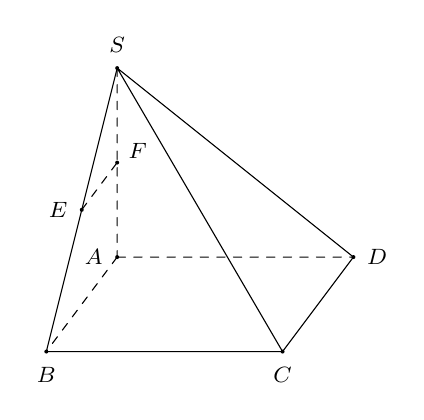
\begin{tikzpicture}[scale=0.6, font=\footnotesize, line join=round, line cap=round, >=stealth]
	\path (0,0)coordinate(A)
	--++(-1.5,-2) coordinate(B)
	--++(5,0) coordinate(C)
	(A)--+(5,0) coordinate (D)
	--+(0,4) coordinate (S);
	\draw (S)--(B)--(C)--(D)--cycle (S)--(C);
	\draw[dashed] (S)--(A) (A)--(B) (A)--(D);
	\foreach \p/\q in {A/180,B/-90,C/-90,D/0,S/90}{
	\path (\p) node[shift={(\q:3mm)}]{$\p$};
	\fill[black] (\p) circle (1.2pt);}
	\path (S)--(A) coordinate[pos=0.5] (F);
	\path (S)--(B) coordinate[pos=0.5] (E);
	\draw[dashed] (E)--(F);
	\path (F) node[shift={(30:3mm)}]{$F$};
	\path (E) node[shift={(180:3mm)}]{$E$};
	\fill[black] (F) circle (1.2pt);
	\fill[black] (E) circle (1.2pt);
	\end{tikzpicture}
	}
	\loigiai{
	\begin{itemize}
		\item Đường thẳng $SC$ và đường thẳng $EF$ chéo nhau.
		\item Ta có $EF$ là đường trung bình của tam giác $SAB$ nên $EF \parallel AB$. Mà $AB \parallel CD$ nên $EF \parallel CD$.
		\item Đường thẳng $AD$ và đường thẳng $SC$ chéo nhau.
		\item Đường thẳng $AE$ và đường thẳng $BF$ cắt nhau.
	\end{itemize}
	}
\end{ex}

\begin{ex}[\textit{Trích đề thi HK1 - trường THPT Nguyễn Gia Thiều - Năm học 2024-2025}]%[1H4H2-2]
	\immini[thm]{Cho hình chóp $S.ABCD$, có đáy $ABCD$ là hình thang, $AD \parallel BC$. Giao tuyến của hai mặt phẳng $(SAD)$ và $(SBC)$ là đường thẳng qua $S$ và}
	{\begin{tikzpicture}
	\def\a{3}
	\path (0:0) coordinate (A)
	++(0:1.7*\a) coordinate (D)
	($(A)+(-70:\a/2)$) coordinate (B)
	($(B)+(D)-(A)$) coordinate (Ct)
	($(B)!.5!(Ct)$) coordinate (C)
	($(A)+(75:0.9*\a)$) coordinate (S)
	;
	\draw[dashed] (D)--(A);
	\draw (A)--(B)--(C)--(D)--(S)--(B) (C)--(S)--(A);
	\foreach \x/\g in {A/180,B/-135,C/-45,D/0,S/90}
	\fill (\x) circle (1pt)
	($(\g:3mm)+(\x)$) node {$\x$}; 
	\end{tikzpicture}}
	\choice
	{qua giao điểm của hai đường thẳng $AC$, $BD$}
	{song song với $AB$}
	{\True song song với $AD$}
	{song song với $AC$}
	\loigiai{
	Do $ABCD$ là hình thang có $AD \parallel BC$ nên giao tuyến của $(SAD)$ và $(SBC)$ là đường thẳng qua $S$ và song song với $AD$ và $BC$.
	}
\end{ex}

\begin{ex}[\textit{Trích đề thi HKI - trường THPT Nguyễn Khuyến - Năm học 2024-2025}]%[1H4H2-2]
	Cho tứ diện $ABCD$. Các điểm $M$, $N$ lần lượt là trung điểm $BD$ và $AD$. Các điểm $H$, $G$ lần lượt là trọng tâm các tam giác $BCD$; $ACD$. Đường thẳng $HG$ chéo với đường thẳng nào sau đây?
	\choice
	{$MN$}
	{\True $CD$}
	{$CN$}
	{$AB$}
	\loigiai{
	\immini{
	Ta có $\heva{&H \in (BCD) \\&G \not\in (BCD)} \Rightarrow G \not\in (HCD)$.\\
	Do đó, bốn điểm $H$, $G$, $C$ và $D$ không đồng phẳng.\\
	Suy ra $HG$ và $CD$ chéo nhau.
	}
	{\begin{tikzpicture}[font=\footnotesize,line join=round, line cap=round, >=stealth,scale=1] 
	\foreach \x/\y/\pos in {0/0/B, 1.5/-2/D, 4/0/C, 2/3/A} \path ($(\x,\y)$) coordinate (\pos); 
	\path ($(B)!1/2!(D)$) coordinate (M) ($(A)!1/2!(D)$) coordinate (N)
	($(C)!1/2!(D)$) coordinate (I) ($(B)!2/3!(I)$) coordinate (H) ($(A)!2/3!(I)$) coordinate (G); 
	\draw[dashed] (I)--(B)--(C) (H)--(G);
	\draw (D)--(A)--(B)--(D)--(C)--(A)--(I) (M)--(N);
	\foreach \x/\pos in {A/90, B/-150, C/-30, D/-90, M/-150, N/0, H/-80, G/30, I/-30} \fill (\x) circle(1pt) node[{shift=(\pos:0.25)}]{$\x$}; 
	\end{tikzpicture}}
	}
\end{ex}

\begin{ex}[\textit{Trích đề thi HKI - trường THPT Nguyễn Thái Bình - Năm học 2024-2025}]%[1H4H2-2]
	Cho hình chóp $S.ABCD$ có đáy $ABCD$ là hình bình hành tâm $O$. Gọi $I$, $J$ lần lượt là trung điểm của $SA$ và $SC$. Đường thẳng $IJ$ song song với đường thẳng nào?
	\choice
	{$BD$}
	{$SO$}
	{\True $AC$}
	{$BC$}
	\loigiai{
	\immini{Xét tam giác $SAC$, ta có
	\begin{itemize}
		\item $I$ là trung điểm cạnh $SA$.
		\item $J$ là trung điểm cạnh $SC$.
	\end{itemize}
	Suy ra $IJ$ là đường trung bình của tam giác $SAC$. Do đó $IJ\parallel AC$.}
	{\begin{tikzpicture}
	\def\a{3}
	\path (0:0) coordinate (A)
	++(0:\a) coordinate (D)
	++(-130:\a/2) coordinate (C)
	($(A)+(C)-(D)$) coordinate (B)
	($(A)+(80:\a)$) coordinate (S)
	($(S)!.5!(A)$) coordinate (I)
	($(S)!.5!(C)$) coordinate (J)
	(intersection of A--C and B--D) coordinate (O);
	\draw[dashed] (B)--(A)--(D)(A)--(S) (A)--(C)(I)--(J) (B)--(D);
	\draw(B)-- (C)--(D)(B)--(S)(C)--(S)(D)--(S);
	\foreach \x/\g in {A/135,B/-135,C/-45,D/45,S/90,O/-90,I/15,J/2}
	\fill[black] (\x) circle (1pt)
	($(\g:3mm)+(\x)$) node {$\x$};
	\end{tikzpicture}}
	}
\end{ex}

\begin{ex}[\textit{Trích đề thi HKI - trường THPT Gia Lộc 2 - Năm học 2024-2025}]%[1H4N2-2] 
	\immini{Cho hình chóp $S.ABCD$ có đáy là hình bình hành. $F$, $G$ lần lượt là trung điểm của $SB$ và $SC$. Hãy chọn khẳng định đúng trong các khẳng định sau?
	\choice
	{\True $FG \parallel A D$}
	{$FG$ và $SA$ cắt nhau}
	{$FG$ và $BC$ chéo nhau}
	{$FG \parallel CD$}}{\begin{tikzpicture}[scale=.75, font=\footnotesize, line join=round, line cap=round, >=stealth]
	\def\a{3}
	\def\b{2.5}
	\def\h{3.5}
	\def\g{35}
	\path
	(0,0) coordinate (A)
	(0:\a) coordinate (B)
	--++(\g:\b) coordinate (C)
	--++(180:\a)coordinate (D)
	;

	\coordinate (S) at ($(D)+(.5,\h)$); 
	\coordinate (G) at ($(C)!1/2!(S)$);
	\coordinate (F) at ($(S)!1/2!(B)$); 

	\draw (S)--(A)--(B)--(C) (B)--(S)--(C) (F)--(G);

	\draw[dashed] (B)--(D)--(S) (A)--(D)--(C)--(A);

	\foreach \x/\g in {A/-90,B/-90,C/0,D/150,S/90,F/180,G/10} \fill (\x) circle (1pt)+(\g:.25)node {$\x$};
	\end{tikzpicture}}
	\loigiai{Ta có $F$, $G$ lần lượt là trung điểm của $SB$ và $SC$ nên $FG$ là đường trung bình trong $\triangle SBC$, suy ra $FG\parallel BC$ mà $BC\parallel AD$ nên $FG\parallel AD$.
	}
\end{ex}

\begin{ex}[\textit{Trích đề thi HKI - trường THPT Thị xã Quảng Trị - Năm học 2024-2025}]%[1H4N2-2]
	Cho hình chóp $S.ABCD$ có đáy $ABCD$ là hình bình hành tâm $O$. Gọi $I$, $J$ lần lượt là trung điểm của $SB$ và $SD$. Đường thẳng $IJ$ song song với đường thẳng nào dưới đây?
	\choice
	{$SO$}
	{$BC$}
	{\True $BD$}
	{$AC$}
	\loigiai{
	\immini
	{Xét tam giác $\Delta SBD$ có $IJ$ là đường trung bình nên $IJ \parallel BD$.}
	{\begin{tikzpicture}[scale=0.6, >=stealth, font=\footnotesize, line join=round, line cap=round]
	\path (0,0) coordinate (A)
	(-1.3,-1.6) coordinate (B)
	(2.5,-1.6) coordinate (C)
	;
	\coordinate (D) at ($(A)+(C)-(B)$);
	\coordinate (S) at ($(A)+(0,3)$);
	\coordinate (h) at ($(A)!0.5!(S)$);
	\coordinate (J) at ($(S)!0.5!(D)$);
	\coordinate (I) at ($(S)!0.5!(B)$);
	\path (intersection of A--C and B--D) coordinate (O);
	\draw (S)--(B)--(C)--(D)--cycle (S)--(C);
	\draw[dashed](A)--(S) (A)--(B) (A)--(D) (A)--(C) (B)--(D) (I)--(J);
	\foreach \p/\r in {S/90,A/180,B/-90,C/-90,D/30,O/-90,J/90,I/135}
	\fill (\p) circle (1pt) node[shift={(\r:3mm)}]{$\p$};
	\end{tikzpicture}}
	}
\end{ex}

\begin{ex}[\textit{Trích đề thi GKI - trường THPT Trần Phú - Năm học 2024-2025}]%[1H4H2-2]
	\immini
	{Cho hình chóp $S.ABCD$ có đáy $ABCD$ là hình bình hành tâm $O$. Gọi $M$, $N$ lần lượt là trung điểm của đoạn thẳng $SA$, $SD$. Khẳng định nào sau đây đúng
	\choice
	{Hai mặt phẳng $(SAD)$ và $(SBC)$ cắt nhau theo 
		$SO$}
	{\True Hai mặt phẳng $(SAD)$ và $(SBC)$ cắt nhau theo giao tuyến là đường thẳng đi qua điểm $S$ và song song với đường thẳng $MN$}
	{Hai mặt phẳng $(SAD)$ và $(SBC)$ cắt nhau theo giao tuyến là đường thẳng đi qua điểm $S$ và song song với hai đường thẳng $MC$, $NB$}
	{Hai mặt phẳng $(SAD)$ và $(SBC)$ cắt nhau theo giao tuyến là đường thẳng đi qua điểm $S$ và song song với hai đường thẳng $AB$, $CD$}
	}
	{\begin{tikzpicture}[line join=round,line cap=round,font=\footnotesize,scale=1]
	\coordinate[label=below left:$B$] (B) at (0,0);
	\coordinate[label=above right:$A$] (A) at (1,1.2);
	\coordinate[label=below right:$C$] (C) at (4,0);
	\coordinate[label=above right:$D$] (D) at ($(C)-(B)+(A)$);
	\coordinate[label=below:$O$] (O) at ($(A)!.5!(C)$);
	\coordinate[label=above left:$S$] (S) at ($(O)+(90:4)$);
	\coordinate[label=below right:$M$] (M) at ($(S)!.5!(A)$);
	\coordinate[label=above right:$N$] (N) at ($(S)!.5!(D)$);
	\draw (B)--(C)--(D)--(S)--cycle (S)--(C);
	\draw[dashed] (C)--(A)--(D)--(B) (O)--(S)--(A)--(B) (M)--(N);
	\fill (A)circle(1pt) (B)circle(1pt) (C)circle(1pt) (D)circle(1pt) (S)circle(1pt) (O)circle(1pt) (M)circle(1pt) (N)circle(1pt);
	\end{tikzpicture}
	}
	\loigiai{
		Khẳng định \lq\lq Hai mặt phẳng $(SAD)$ và $(SBC)$ cắt nhau theo giao tuyến là đường thẳng đi qua điểm $S$ và song song với đường thẳng $MN$\rq\rq\ đúng.
	}
\end{ex}

\begin{ex}[\textit{Trích đề thi HKI - trường THPT Mạc Đỉnh Chi - Năm học 2024-2025}]%[1H4H2-2]
	Cho hình chóp $S.ABCD$ có đáy là hình bình hành tâm $O$. Gọi $M$, $N$, $P$ lần lượt là trung điểm của $AB$, $SB$ và $SC$. Khẳng định nào sau đây là đúng?
	\choice
	{$MN\parallel SO$}
	{$MN\parallel SC$}
	{$MN\parallel SD$}
	{\True $MN\parallel OP$}
	\loigiai{
	\immini
	{Ta có $ MN $ là đường trung bình $ \triangle SAB $.\\
	Suy ra $ MN \parallel SA $. \quad $ (1) $\\
	Hơn nữa $ OP $ là đường trung bình $ \triangle SAC $.\\
	Suy ra $ OP \parallel SA $. \quad $ (2) $\\
	Từ $ (1) $ và $ (2) $ suy ra $ MN \parallel OP \parallel SA $.}
	{\begin{tikzpicture}[line join=round,line cap=round,font=\footnotesize,scale=.9]
	\coordinate[label=below left:$B$] (B) at (0,0);
	\coordinate[label=above right:$A$] (A) at (1,1.2);
	\coordinate[label=below right:$C$] (C) at (4,0);
	\coordinate[label=above right:$D$] (D) at ($(C)-(B)+(A)$);
	\coordinate[label=below:$O$] (O) at ($(A)!.5!(C)$);
	\coordinate[label=above left:$S$] (S) at ($(O)+(90:4)$);
	\coordinate[label=right:$M$] (M) at ($(A)!1/2!(B)$);
	\coordinate[label=above left:$N$] (N) at ($(S)!1/2!(B)$);
	\coordinate[label=right:$P$] (P) at ($(S)!1/2!(C)$);
	\draw (B)--(C)--(D)--(S)--cycle (S)--(C) (N)--(P);
	\draw[dashed] (C)--(A)--(D)--(B) (O)--(S)--(A)--(B) (O)--(P)--(M)--(N);
	\fill (A)circle(1pt) (B)circle(1pt) (C)circle(1pt) (D)circle(1pt) (S)circle(1pt) (O)circle(1pt) (P)circle(1pt) (M)circle(1pt) (N)circle(1pt);
	\end{tikzpicture}}
	}
\end{ex}

\begin{ex}[\textit{Trích đề thi GKI - trường THPT Trần Phú - Năm học 2024-2025}]%[1H4H2-3]
	\immini
	{Cho hình chóp $S.ABCD$ có đáy $ABCD$ là hình bình hành tâm $O$. Gọi $M$, $N$ lần lượt là trung điểm $SA$, $SD$. Khẳng định nào sau đây \textbf{sai}
	\choice
	{Hai đường thẳng $MN$ và $BC$ song song nhau}
	{Hai đường thẳng $ON$ và $SB$ song song nhau}
	{Hai đường thẳng $OM$ và $SC$ song song nhau}
	{\True Hai mặt phẳng $(SAB)$ và $(SCD)$ cắt nhau theo giao tuyến là đường thẳng đi qua điểm $S$ và song song với hai đường thẳng $MB$, $NC$}
	}
	{\begin{tikzpicture}[line join=round,line cap=round,font=\footnotesize,scale=1]
	\coordinate[label=below left:$B$] (B) at (0,0);
	\coordinate[label=above right:$A$] (A) at (1,1);
	\coordinate[label=below right:$C$] (C) at (4,0);
	\coordinate[label=above right:$D$] (D) at ($(C)-(B)+(A)$);
	\coordinate[label=below:$O$] (O) at ($(A)!.5!(C)$);
	\coordinate[label=above left:$S$] (S) at ($(O)+(90:4)$);
	\coordinate[label=below right:$M$] (M) at ($(S)!.5!(A)$);
	\coordinate[label=above right:$N$] (N) at ($(S)!.5!(D)$);
	\draw (B)--(C)--(D)--(S)--cycle (S)--(C);
	\draw[dashed] (C)--(A)--(D)--(B) (O)--(S)--(A)--(B) (M)--(N)--(O)--cycle;
	\fill (A)circle(1pt) (B)circle(1pt) (C)circle(1pt) (D)circle(1pt) (S)circle(1pt) (O)circle(1pt) (M)circle(1pt) (N)circle(1pt);
	\end{tikzpicture}}
	\loigiai{
	Hai mặt phẳng $(SAB)$, $(SCD)$ phân biệt, có điểm chung $S$, lần lượt chứa hai đường thẳng song song là $AB$, $CD$ nên giao tuyến của chúng là một đường thẳng $d$ đi qua $S$ và song song với $AB$, $CD$. Do đó, khẳng định \lq\lq Hai mặt phẳng $(SAB)$ và $(SCD)$ cắt nhau theo giao tuyến là đường thẳng đi qua điểm $S$ và song song với hai đường thẳng $MB$, $NC$\rq\rq\ là sai.
	}
\end{ex}

\begin{ex}[\textit{Trích đề thi HKI - trường THPT Mạc Đỉnh Chi - Năm học 2024-2025}]%[1H4H2-3]
	Cho hình chóp $S.ABCD$. Gọi $M$, $N$ lần lượt là trung điểm của $SD$ và $CD$. Giao tuyến của hai mặt phẳng $(BMN)$ và $(SBC)$ là đường thẳng nào sau đây?
	\choice
	{\True Đường thẳng qua $B$ và song song với $SC$}
	{Đường thẳng qua $B$ và song song với $SD$}
	{Đường thẳng qua $B$ và song song với $SA$}
	{Đường thẳng qua $B$ và song song với $CD$}
	\loigiai{
	\immini
	{Do $ MN $ là đường trung bình tam giác $ SCD $ nên $ MN \parallel SC $.\\
	Ta có $ \heva{&B\in (SBC)\cap (BMN)\\&MN \parallel SC\\&MN \subset (BMN),\,SC\subset (SBC).} $
	Suy ra $ (SBC)\cap (BMN)= Bx \parallel SC $.}
	{\begin{tikzpicture}[line join=round,line cap=round,font=\footnotesize,scale=1]
	\coordinate[label=left:$A$] (A) at (0,0);
	\coordinate[label=below left:$B$] (B) at (.5,-1);
	\coordinate[label=below right:$C$] (C) at (2.6,-.8);
	\coordinate[label=right:$D$] (D) at (4,0);
	\coordinate[label=above left:$S$] (S) at (1.2,3);
	\coordinate[label=right:$M$] (M) at ($(S)!1/2!(D)$);
	\coordinate[label=below:$N$] (N) at ($(C)!1/2!(D)$);
	\draw (A)--(B)--(C)--(D)--(S)--cycle (B)--(S)--(C) (M)--(N);
	\draw[dashed] (A)--(D) (N)--(B)--(M);
	\fill (A)circle(1pt) (B)circle(1pt) (C)circle(1pt) (D)circle(1pt) (S)circle(1pt) (M)circle(1pt) (N)circle(1pt);
	\end{tikzpicture}}
	}
\end{ex}

\begin{ex}[\textit{Trích đề thi GKI - trường THPT Võ Thị Sáu - Năm học 2024-2025}]%[1H4N2-2]
	Cho hình chóp $S. ABCD$ có đáy $ABCD$ là hình bình hành tâm $O$. Gọi $M, N$ lần lượt là trung điểm $SA, SB$ và $P$ điểm bất kì trên cạnh $SC$ (không trùng với trung điểm). Trong các mệnh đề sau, mệnh đề nào \textbf{sai}?
	\choice
	{$ON$ song song $SD$}
	{\True $MP$ song song $AC$}
	{$OM$ song song $SC$}
	{$MN$ song song $CD$}
	\loigiai{
	\immini
	{Ta có $MP$ không song song $AC$ vì trong tam giác $SAC$ có $M$ là trung điểm $SA$ và $P$ không là trung điểm $SC$.}
	{\begin{tikzpicture}
	\def\a{3}
	\path (0:0) coordinate (A)
	++(0:\a) coordinate (D)
	++(-130:\a/2) coordinate (C)
	($(A)+(C)-(D)$) coordinate (B)
	($(A)+(80:\a)$) coordinate (S)
	($(S)!.5!(A)$) coordinate (M)
	($(S)!.6!(C)$) coordinate (P)
	($(S)!.5!(B)$) coordinate (N)
	(intersection of A--C and B--D) coordinate (O);
	\draw[dashed] (B)--(A)--(D)(A)--(S) (A)--(C)(N)--(M)--(P) (B)--(D) (M)--(O) (N)--(O) ;
	\draw(B)-- (C)--(D)(B)--(S)(C)--(S)(D)--(S);
	\foreach \x/\g in {A/135,B/-135,C/-45,D/45,S/90,O/-90,M/15,P/2,N/180}
	\fill[black] (\x) circle (1pt)
	($(\g:3mm)+(\x)$) node {$\x$};
	\end{tikzpicture}}
	}
\end{ex}

\begin{ex}[\textit{Trích đề thi GKI - trường THPT Vàm Đình - Năm học 2023-2024}]%[1H4H2-3]
	Cho hình chóp $S.ABCD$ có đáy $ABCD$ là hình bình hành. Gọi $d$ là giao tuyến của hai mặt phẳng $(SAD)$ và $(SBC)$. Khẳng định nào dưới đây đúng?
	\choice
	{$d$ đi qua $S$ và song song với $BD$}
	{$d$ đi qua $S$ và song song với $CD$}
	{\True $d$ đi qua $S$ và song song với $BC$}
	{$d$ đi qua $S$ và song song với $AB$}
	\loigiai{
	\immini
	{Hai mặt phẳng $(SAD)$ và $(SBC)$ có điểm chung $S$, lần lượt đi qua hai đường thẳng song song với nhau là $AD$ và $BC$, nên giao tuyến của hai mặt phẳng $(SAD)$ và $(SBC)$ là $d$ đi qua $S$ và song song với $BC$.}
	{\begin{tikzpicture}[font=\footnotesize, line join=round, line cap=round, >=stealth,scale=0.7]
	\def\x{2}
	\def\y{4}
	\def\h{3}
	\path 
	(0:0) coordinate (A)
	(-120:\x) coordinate (B)
	(0:\y) coordinate (D)
	(90:\h) coordinate (S)
	($(B)+(D)-(A) $) coordinate (C)
	($(S)+(180:1)$)coordinate (d1)
	($(S)+(0:4)$)coordinate (d2)
	;
	\draw (d1)--(d2) node[above]{$d$};
	\draw (B)--(C)--(D) (S)--(B) (S)--(C) (S)--(D);
	\draw[dashed] (B)--(A)--(D) (S)--(A);
	\foreach \x/\g in{A/-90,B/-90,C/-90,D/-80,S/90}
	\fill[black](\x) circle (1pt)
	($(\x)+(\g:5mm)$) node{$\x$};
	\end{tikzpicture}}
	}
\end{ex}
\begin{ex}[\textit{Trích đề thi GKI - trường THPT Chuyên Hùng Vương - Năm học 2023-2024}]%[1H4H2-2]
	Cho tứ diện $ABCD$. Gọi $M$, $N$ lần lượt là trung điểm của các đoạn thẳng $AB$, $AD$. Giao tuyến của hai mặt phẳng $(CMN)$ và $(BCD)$ là đường thẳng song song với đường thẳng nào sau đây?
	\choice
	{$AB$}
	{$AC$}
	{$AD$}
	{\True $BD$}
	\loigiai{
	\immini
	{Nhận thấy rằng $MN$ là đường trung bình trong tam giác $ABD$ do đó $MN\parallel BD$.\\
	Hai mặt phẳng $(MNC)$ và $(BDC)$ có một điểm chung là $C$ và lần lượt chứa hai đường thẳng song song $MN$, $DB$ với nhau do đó giao tuyến của chúng là đường thẳng đi qua $C$ và song song với $BD$.}
	{\begin{tikzpicture}[scale=1, font=\footnotesize, line join=round, line cap=round, >=stealth]
	\path
	(0,0) coordinate (B) node[left]{$B$}
	(4,0) coordinate (D) node[right]{$D$}
	(1,3) coordinate (A) node[above]{$A$}
	(2,-1) coordinate (C) node[below]{$C$}
	($(A)!0.5!(B)$) coordinate (M) node[above left]{$M$}
	($(A)!0.5!(D)$) coordinate (N) node[above right]{$N$}
	;
	\draw (A)--(B)--(C)--(D)--cycle (A)--(C) (M)--(C)--(N);
	\draw[dashed] (B)--(D) (M)--(N);
	\draw[fill=black] (M) circle (1pt) (N) circle (1pt);
	\end{tikzpicture}}
	}
\end{ex}

\begin{ex}[\textit{Trích đề thi GKI - trường THPT Lê Quý Đôn - Năm học 2023-2024}]%[1H4H2-5]
	\immini[thm]
	{Cho tứ diện $ABCD$ và điểm $M$ ở trên cạnh $BC$. Mặt phẳng $(\alpha)$ qua $M$ song song song với $AB$ và $CD$ cắt $AC$, $AD$ và $BD$ lần lượt tại $N$, $P$, $Q$. Tứ giác $MNPQ$ là hình gì?
	\choice
	{Hình thoi}
	{Hình thang}
	{\True Hình bình hành}
	{Hình chữ nhật}
	}
	{\begin{tikzpicture}[declare function={r=3;},scale=0.7]
	\path (0,0) coordinate (B)
	(2,4) coordinate (A)
	(3,-2) coordinate (C)
	(5,0) coordinate (D)
	(1.5,-1) coordinate (M);
	\draw (A)--(B)--(C)--cycle;
	\draw [dashed](B)--(D);
	\draw (A)--(C)--(D)--cycle;
	\foreach \t/\g in {A/90,B/180,C/-90,D/0,M/210}{
	\draw[fill=white] (\t) circle (1pt) node[shift={(\g:10pt)},font=\normalsize]{$ \t $};
	}
	\end{tikzpicture}}
	\loigiai{
	\immini
	{Trong mặt phẳng $(ABC)$ qua $M$ kẻ đường thẳng song song với $AB$ cắt $BC$ tại $N$.\\
	Trong mặt phẳng $(ACD)$ qua $N$ kẻ đường thẳng song song với $CD$ cắt $AD$ tại $P$.\\
	Trong mặt phẳng $(ABD)$ qua $P$ kẻ đường thẳng song song với $AB$ cắt $BD$ tại $Q$.\\
	Khi đó mặt phẳng $(\alpha)$ là mặt phẳng $(MNPQ)$.\\
	Ta có $\heva{&MN \parallel AB\\&PQ \parallel AB} \Rightarrow MN \parallel PQ$.\\
	Ta có $\heva{&MQ \parallel CD\\&NP \parallel CD} \Rightarrow MQ \parallel NP$.\\
	Vậy $MNPQ$ là hình bình hành.}
	{\begin{tikzpicture}[declare function={r=3;},scale=0.7]
	\path (0,0) coordinate (B)
	(2,4) coordinate (A)
	(3,-2) coordinate (C)
	(5,0) coordinate (D)
	(1.5,-1) coordinate (M);
	\path ($(A)!0.5!(C)$) coordinate (N);
	\path ($(A)!0.5!(D)$) coordinate (P);
	\path ($(B)!0.5!(D)$) coordinate (Q);
	\draw (A)--(B)--(C)--cycle (M)--(N)--(P);
	\draw [dashed](B)--(D) (M)--(Q)--(P);
	\draw (A)--(C)--(D)--cycle;
	\foreach \t/\g in {A/90,B/180,C/-90,D/0,M/230,P/30,N/160,Q/-90}{
	\fill (\t) circle (1pt) node[shift={(\g:10pt)}]{$\t$};
	}
	\end{tikzpicture}}
	}
\end{ex}

\begin{ex}[\textit{Trích đề thi GKI - trường THPT Nguyễn Trãi - Năm học 2023-2024}]%[1H4H2-2]
	Cho tứ diện $ABCD$. Gọi $I$, $J$ lần lượt là trọng tâm tam giác $ABD$ và tam giác $ABC$. Chọn khẳng định đúng trong các khẳng định sau?
	\choice
	{\True $IJ$ song song với $CD$}
	{$IJ$ song song với $AB$}
	{$IJ$ chéo $CD$}
	{$IJ$ cắt $AB$}
	\loigiai{
	\immini
	{Gọi $M$, $N$ lần lượt là trung điểm của $BD$ và $BC$.\\
	Ta có $\dfrac{AI}{AM}=\dfrac{AJ}{AN}=\dfrac{2}{3}\Rightarrow IJ\parallel MN$. \quad$(1)$\\
	Trong tam giác $ABC$ ta có\\ $\dfrac{BM}{BD}=\dfrac{BN}{BC}=\dfrac{1}{2}\Rightarrow MN\parallel CD$. \quad$(2)$.\\
	Từ $(1)$ và $(2)$ suy ra $IJ\parallel CD$.}
	{\begin{tikzpicture}[line join = round, line cap = round,>=stealth,font=\footnotesize,scale=1,declare function={bd=4.5;bc=2.5; gocB=-60;ha=3;}]
	\path 
	(0,0) coordinate (B)
	(bd,0) coordinate (D)
	(gocB:bc) coordinate (C)
	(70:ha) coordinate (A)
	($(B)!.5!(D)$) coordinate (M)
	($(B)!.5!(C)$) coordinate (N)
	($(A)!2/3!(M)$) coordinate (I)
	($(A)!2/3!(N)$) coordinate (J)
	;
	\draw (A)--(B)--(C)--(D)--cycle (A)--(C) (A)--(N);
	\draw[dashed] (B)--(D) (A)--(M)--(N) (I)--(J);
	\foreach \x/\gm in {A/90,B/180,C/-90,D/0,I/0,J/180,M/-90,N/-120} \fill (\x) circle (1pt) ($(\x)+(\gm:3.5mm)$)node{$\x$};
	\end{tikzpicture}}
	}
\end{ex}

\begin{ex}[\textit{Trích đề thi GKI - trường THPT Lê Quý Đôn - Năm học 2023-2024}]%[1H4V2-4]
	Cho hình chóp $S.ABCD$ có đáy $ABCD$ là hình bình hành, $E$ là điểm thuộc cạnh bên $SD$ sao cho $SD=3SE$. Giao điểm của $SA$ và mặt phẳng $\left(BCE\right)$ là điểm $F$. Khẳng định nào dưới đây đúng?
	\choice
	{$F$ không tồn tại}
	{$BCEF$ là hình thang có đáy lớn gấp 2 lần đáy nhỏ}
	{$BCEF$ là hình bình hành}
	{\True $FA=2SF$}
	\loigiai{
	\immini
	{Gọi $d=(EBC)\cap (SAD)$.\\
	Ta có
	$\heva{&BC \subset (EBC),AD\subset (SAD) \\&BC\parallel AD \\&E\in (EBC)\cap (SAD)}\\
	\Rightarrow \heva{&E\in d \\&d\parallel BC\parallel AD.}$ \\
	Trong mặt phẳng $(SAD)$, qua điểm $E$ kẻ $d \parallel AD$, \\ $d \cap SA =F$. Khi đó $F= SA \cap (EBC)$.\\
	Áp dụng định lí Thalès trong tam giác $SAD$ với\\ $EF \parallel AD$, ta có $\dfrac{SF}{FA} =\dfrac{SE}{ED}=\dfrac{1}{2}$.\\ 
	Do đó $FA=2SF$.}
	{\begin{tikzpicture}[scale=1,>=stealth, font=\footnotesize, line join=round, line cap=round]
	\path 
	(0,0) coordinate (A)
	(-1.9,-1.6) coordinate (B)
	(1.8,-1.6) coordinate (C)
	(0,3.5) coordinate (S)
	;
	\coordinate (D) at ($(A)+(C)-(B)$);
	\coordinate (E) at ($(S)!1/3!(D)$);
	\coordinate (F) at ($(S)!1/3!(A)$);
	\draw (S)--(B)--(C)--(D)--cycle (S)--(C) (E)--(C) ;
	\draw[dashed](A)--(S) (C)--(A)--(B) (A)--(D) (B)--(D) (B)--(E) (E)--(F)(B)--(F);
	\foreach \p/\r in {S/90,A/180,D/0,B/-90,C/-90,E/70,F/135}
	\fill (\p) circle (1pt) node[shift={(\r:3mm)}]{$\p$};
	\end{tikzpicture}}
	}
	\end{ex}
\Closesolutionfile{ans}

\ind{PHẦN II.} \inden{Câu trắc nghiệm đúng sai. Trong mỗi ý a), b), c), d) ở mỗi câu, học sinh chọn đúng hoặc sai.}
\setcounter{ex}{0}
\Opensolutionfile{ans}[ans/1D1-Bai1-2-DS]
	\begin{ex}%[1H4N2-1]
	Trong không gian.
	\choiceTF
	{Hai đường thẳng không có điểm chung thì chúng song song với nhau}
	{Hai đường thẳng không có điểm chung thì chúng chéo nhau}
	{Hai đường thẳng có điểm chung thì chúng cắt nhau}
	{\True Hai đường thẳng không thể cùng nằm trên một mặt phẳng thì chúng chéo nhau}
	\loigiai{
	\begin{itemchoice}
		\itemch Hai đường thẳng không có điểm chung thì có thể là chúng có thể chéo nhau.
		\itemch Hai đường thẳng không có điểm chung thì có thể là chúng có thể song song.
		\itemch Hai đường có điểm chung thì chúng có thể cắt nhau hoặc trùng nhau.
		\itemch Hai đường thẳng không thể cùng nằm trên một mặt phẳng thì chúng chéo nhau.
	\end{itemchoice}
	}
\end{ex}

\begin{ex}%[1H4N2-2]
	Cho hình chóp $S.ABCD$ có đáy là hình bình hành.
	\choiceTF
	{\True $AB$ song song $CD$}
	{\True $SA$ cắt $SC$}
	{$SA$ song song $BC$}
	{\True $SC$ chéo nhau $AB$}
	\loigiai{
	\begin{center}
	\begin{tikzpicture}[font=\footnotesize, line join=round, line cap=round, >=stealth, scale=1]
	\path (0,0) coordinate (A) (-150:1.5) coordinate (B) (3,0) coordinate (D) ($(B)+(3,0)$) coordinate (C) (1,2) coordinate (S);
	\draw (S)--(B)--(C)--(D)--cycle (S)--(C);
	\draw[dashed] (B)--(A)--(D) (S)--(A);
	\foreach \x/\g in {S/90, A/135, B/-135, C/-45, D/45}{\fill (\x) circle (1pt)+(\g:0.3)node{$\x$};}
	\end{tikzpicture}
	\end{center}
	\begin{itemchoice}
		\itemch Do $ABCD$ là hình bình hành nên $AB\parallel CD$.
		\itemch Hai đường thẳng $SA$ và $SC$ cắt nhau tại $S$.
		\itemch Hai đường thẳng $SA$ và $BC$ không đồng phẳng. Vì vậy $SA$ và $BC$ là hai đường thẳng chéo nhau.
		\itemch Hai đường thẳng $SC$ và $AB$ không đồng phẳng. Vì vậy $SC$ và $AB$ là hai đường thẳng chéo nhau.
	\end{itemchoice}
	}
\end{ex}

\begin{ex}%[1H4V2-2]
	Cho tứ diện $ABCD$ có $I$, $J$ theo thứ tự là trung điểm của các cạnh $BC$, $BD$. Gọi $(P)$ là mặt phẳng qua $I$, $J$ và cắt các cạnh $AC$, $AD$ lần lượt tại hai điểm $M$, $N$.
	\choiceTF
	{\True $IJ=\dfrac{1}{2}CD$}
	{$MN$ cắt $DC$}
	{\True $IJNM$ là một hình thang}
	{\True Nếu $M$ là trung điểm của đoạn $AC$ thì $IJNM$ là hình bình hành}
	\loigiai{
	\begin{center}
	\begin{tikzpicture}[font=\footnotesize, line join=round, line cap=round, >=stealth, scale=1]
	\path (0,0) coordinate (B) (-25:3) coordinate (C) (4,0) coordinate (D) (1,3) coordinate (A)
	($(B)!1/2!(C)$) coordinate (I)
	($(B)!1/2!(D)$) coordinate (J)
	($(A)!1/3!(C)$) coordinate (M)
	($(A)!1/3!(D)$) coordinate (N);
	\draw (A)--(B)--(C)--(D)--cycle (A)--(C) (I)--(M)--(N);
	\draw[dashed] (B)--(D) (I)--(J)--(N);
	\foreach \x/\g in {A/90, B/135, C/-90, D/45, I/-135, J/-90, M/180, N/45}{\fill (\x) circle (1pt)+(\g:0.3)node{$\x$};}
	\end{tikzpicture}
	\end{center}
	\begin{itemchoice}
		\itemch Ta có $IJ$ là đường trung bình của tam giác $BCD$ nên $IJ\parallel CD$ và $IJ=\dfrac{1}{2}CD$.
		\itemch Ta có $(P)\cap(ACD)=MN$.\\
		Đồng thời $\heva{&IJ\subset (P)\\&CD\subset(ACD)\\&IJ\parallel CD}$.\\
		Suy ra $MN\parallel IJ \parallel CD$.\\
		Do đó $MN$ không cắt $CD$.
		\itemch Ta có $IJ\parallel MN$ nên $IJNM$ là hình thang.
		\itemch Nếu $M$ là trung điểm $AD$. Ta có $MN\parallel AC$ nên $MN$ là đường trung bình của tam giác $ACD$.\\
		Khi đó $MN=\dfrac{1}{2}CD=IJ$.\\
		Xét tứ giác $IJNM$ ta có $MN\parallel IJ$ và $MN=IJ$, suy ra $IJNM$ là hình bình hành.
	\end{itemchoice}
	}
\end{ex}

\begin{ex}%[1H4H2-3]
	Cho hình chóp $S.ABCD$ có đáy là hình bình hành. Điểm $M$ thuộc cạnh $SA$, điểm $E$ và $F$ lần lượt là trung điểm của $AB$ và $BC$.
	\choiceTF
	{\True $EF\parallel AC$}
	{Giao tuyến của hai mặt phẳng $(SAB)$ và $(SCD)$ là đường thẳng qua $S$ và song song với $AC$}
	{\True Giao tuyến của hai mặt phẳng $(MBC)$ và $(SAD)$ đường thẳng qua $M$ và song song với $BC$}
	{\True Giao tuyến của hai mặt phẳng $(MEF)$ và $(SAC)$ là đường thẳng qua $M$ và song song với $AC$}
	\loigiai{
	\begin{center}
	\begin{tikzpicture}[font=\footnotesize, line join=round, line cap=round, >=stealth, scale=1]
	\path (0,0) coordinate (A) (-150:2) coordinate (B) (3,0) coordinate (D) ($(B)+(3,0)$) coordinate (C) (0.5,2) coordinate (S)
	($(S)!1/2!(A)$) coordinate (M)
	($(A)!1/2!(B)$) coordinate (E) ($(B)!1/2!(C)$) coordinate (F)
	($(M)+(0:0.1)$) coordinate (m)
	(intersection of M--m and S--D) coordinate (msd) (intersection of M--m and S--B) coordinate (msb)
	($(S)!1/2!(C)$) coordinate (msc) (intersection of M--msc and S--B) coordinate (msa)
	;
	\draw (S)--(B)--(C)--(D)--cycle (S)--(C)
	(S)--+(-150:2.5)--+(30:1)node[above]{$x$}
	(msd)--+(0:2)node[above]{$y$} (msb)--+(180:1.5)
	(msc)--($(msc)!-1.8!(msa)$)node[above]{$t$} (msa)--($(msa)!-1!(msc)$);
	\draw[dashed] (B)--(A)--(D) (S)--(A)--(C) (M)--(E)--(F)--cycle (M)--(C)
	(msb)--(msd) (msc)--(msa)
	;
	\foreach \x/\g in {S/90, A/135, B/-135, C/-45, D/45, M/35, E/90, F/-90}{\fill (\x) circle (1pt)+(\g:0.3)node{$\x$};}
	\end{tikzpicture}
	\end{center}
	\begin{itemchoice}
		\itemch Xét $\triangle ABC$ có $EF$ là đường trung bình, suy ra $EF\parallel AC$.
		\itemch Xét hai mặt phẳng $(SAB)$ và $(SCD)$ ta có $S\in(SAB)\cap(SCD)$.\\
		Ta có $\heva{&AB\subset (SAB)\\&CD\subset (SCD)\\&AB\parallel CD.}$\\
		Suy ra $Sx=(SAB)\cap (SCD)$, với $Sx$ là đường thẳng qua $S$ và $Sx\parallel AB\parallel CD$.
		\itemch Xét hai mặt phẳng $(MBC)$ và $(SAD)$ ta có $M\in(MAC)\cap(SAD)$.\\
		Ta có $\heva{&BC\subset (MBC)\\&AD\subset (SAD)\\&BC\parallel AD.}$\\
		Suy ra $My=(MBC)\cap (SAD)$, với $My$ là đường thẳng qua $M$ và $My\parallel BC\parallel AD$.
		\itemch Xét hai mặt phẳng $(MEF)$ và $(SAC)$ ta có $M\in(MEF)\cap(SAC)$.\\
		Xét tam giác $ABC$, ta có $EF$ là đường trung bình $\Rightarrow EF\parallel AC$.\\
		Khi đó $\heva{&EF\subset (MEF)\\&AC\subset (SAC)\\&EF\parallel AC.}$\\
		Suy ra $Mt=(MEF)\cap (SAC)$, với $Mt$ là đường thẳng qua $M$ và $Mt\parallel EF\parallel AC$.
	\end{itemchoice}
	}
\end{ex}

\begin{ex}[\textit{Trích đề thi HKI - trường THPT Phạm Phú Thứ - Năm học 2024-2025}]%[1H4H2-4]
	Cho hình chóp tam giác $S.ABC$. Gọi $M$, $N$, $P$ lần lượt là trung điểm của $BC$, $SA$ và $AC$.
	\choiceTF
	{Hai đường thẳng $SC$ và $AB$ có đúng $1$ điểm chung}
	{Điểm $M$ thuộc mặt phẳng $(SAB)$}
	{\True Giao tuyến của $(SBC)$ và $(SAM)$ là đường thẳng $SM$}
	{\True Giao điểm của $MN$ và $(SBP)$ là giao điểm của $MN$ và $SG$, $G$ là trọng tâm $\triangle ABC$}
	\loigiai{
	\begin{center}
	\begin{tikzpicture}
	\def\a{5}
	\def\h{5}
	\path (0:0) coordinate (A)
	++(0:\a) coordinate (B)
	++(-150:4*\a/5) coordinate (C)
	($(C)!0.5!(B)$) coordinate (M)
	($(C)!2/3!(M)$) coordinate (H)
	($(H)+(90:\h)$) coordinate (S)
	($(A)!0.5!(S)$) coordinate (N)
	($(A)!0.5!(C)$) coordinate (P)
	(intersection of A--M and B--P) coordinate (G)
	(intersection of N--M and S--G) coordinate (K);
	\draw (C)--(A) (C)--(B)
	(A)--(S)(B)--(S)--(P)(C)--(S)--(M) ;
	\draw[dashed] (A)--(B)--(P) (C)--(M)--(A) (M)--(N) (S)--(G);
	\foreach \x / \goc in {A/180,B/0,C/-135,M/-30,S/90,N/180,P/180,G/-90,K/0}
	\fill (\x) circle (1pt)+(\goc:0.3) node {$\x$};
	\end{tikzpicture}
	\end{center}
	\begin{itemchoice}
		\itemch Trong hình chóp tam giác 
		$S.ABC$, các đường thẳng $SC$ và $AB$
		không cùng nằm trên một mặt phẳng nên không có điểm chung.
		\itemch $M$ là trung điểm của $BC$. Nếu $M$ thuộc $(SAB)$ thì $BC\in(SAB)$, điều này không đúng vì $BC$ là một cạnh của $\triangle ABC$. 
		\itemch Ta có $\heva{&S\in SM \subset (SAM)\\&S\in SB \subset(SBC)}\Rightarrow S\in (SAM)\cap(SBC)$.\\
		Lại có $\heva{&M\in BC\subset(SBC)\\&M\in SM\subset(SAM)}\Rightarrow M\in (SAM)\cap(SBC)$.\\
		Từ đó suy ra giao tuyến của $(SBC)$ và $(SAM)$ là đường thẳng $SM$.
		\itemch Ta có $MN \subset ( SAM)$, $SG \subset (SAM)$ nên $MN$ và $SG$ giao nhau.\\
		Giả sử trong mặt phẳng $(SAM)$, ta có $K=MN\cap SG$.\quad$(1)$\\
		Ta có $\heva{&S \in (SAM)\\&S\in (SBP)\\&G\in AM\subset (SAM)\\&G\in BP \subset (SBP)}\Rightarrow$
		$SG$ là giao tuyến của $(SAM)$ và $(SBP)$.\\
		Lại có $\heva{&K\in MN\\&K \in SG \subset (SBP)}\Rightarrow K=MN\cap(SBP)$.\quad $(2)$\\
		Từ $(1)$ và $(2)$ ta có giao điểm của $MN$ và $(SBP)$ là giao điểm của $MN$ và $SG$, $G$ là trọng tâm $\triangle ABC$.
	\end{itemchoice}
	}
\end{ex}

\Closesolutionfile{ans}

\ind{PHẦN III.} \inden{Câu trắc nghiệm trả lời ngắn. Mỗi câu học sinh ghi đáp án vào vào ô.}
\setcounter{ex}{0}
\Opensolutionfile{ans}[ans/1D1-Bai1-2-TLN]
\begin{ex}[\textit{Trích đề thi HKI - trường THPT Nguyễn Gia Thiều - Năm học 2024-2025}]%[1H4H2-2]
	Cho tứ diện $ABCD$. Gọi $Q$, $H$ lần lượt là hai trọng tâm hai tam giác $ABC$, $ACD$. Tính $\dfrac{QH}{BD}$ ({\it không làm tròn các phép tính trung gian, chỉ làm tròn kết quả cuối cùng đến hàng phần trăm}).
	\par\shortans{$0{,}33$}
	\loigiai{
	\immini
	{Gọi $M$ là trung điểm của $AC$.\\
	Vì $Q$, $H$ lần lượt là hai trọng tâm hai tam giác $ABC$, $ACD$ nên $\dfrac{MQ}{MB}=\dfrac{1}{3}$ và $\dfrac{MH}{MD}=\dfrac{1}{3}$.\\
	Xét $\triangle MBD$ có $\dfrac{MQ}{MB}=\dfrac{MH}{MD}=\dfrac{1}{3}\Rightarrow QH\parallel BD$ và $\dfrac{QH}{BD}=\dfrac{1}{3}=0{,}33$.}
	{\begin{tikzpicture}[scale=0.8, font=\footnotesize, line join=round, line cap=round, >=stealth]
	\coordinate (B) at (0,0);\coordinate (C) at (2,-1); \coordinate (D) at (6,0);
	\coordinate (A) at ($(B)+(1,4)$);\coordinate (A) at ($(B)+(2,5)$);
	\coordinate (M) at ($(C)!1/2!(A)$); 
	\coordinate (Q) at ($(B)!2/3!(M)$); 
	\coordinate (H) at ($(D)!2/3!(M)$);
	\draw (A)--(B)--(C)--(D)--(A)--(C) (D)--(M) (B)--(M);
	\draw[dashed] (B)--(D) (Q)--(H);
	\foreach \x/\g in {A/90,B/180,C/-90,D/0,Q/-90,H/-90,M/30} \fill[black](\x) circle (1pt) ($(\x)+(\g:3mm)$) node{$\x$};
	\end{tikzpicture}}
	}
\end{ex}

\begin{ex}[\textit{Trích đề thi HKI - trường THPT Nguyễn Gia Thiều - Năm học 2024-2025}]%[1H4H2-3]
	\immini[thm]
	{Cho hình chóp $S.ABCD$, có đáy $ABCD$ (tham khảo hình bên).
	Gọi $M$ là trung điểm của cạnh $BC$ và $AM\parallel CD$, $I$ là điểm thuộc cạnh $SC$ sao cho $IC=2IS$. Đường thẳng $SD$ cắt mặt phẳng $(IMA)$ tại $H$. Tính tỉ số $\dfrac{SH}{HD}$.}
	{\begin{tikzpicture}[scale=0.7, font=\footnotesize, line join=round, line cap=round, >=stealth]
	\coordinate (A) at (0,0);
	\coordinate (B) at (-2,2);
	\coordinate (D) at (2.5,-1);
	\coordinate (C) at (5,2);
	\coordinate (M) at ($(B)!1/2!(C)$);
	\coordinate (S) at ($(A)+(1.5,6)$);
	\coordinate (I) at ($(S)!1/3!(C)$);
	\draw(S)--(B)--(A)--(D)--(C)--(S)--(D) (S)--(A);
	\draw[dashed](B)--(C);
	\foreach \i/\g in {S/90,A/-90,B/180,C/0,D/-90,M/-70,I/60}{\draw[fill=black](\i) circle (1pt) ($(\i)+(\g:3mm)$) node[scale=1]{$\i$};}
	\end{tikzpicture}}
	\par\shortans{$0{,}5$}
	\loigiai{
	\immini
	{Ta có $\heva{&AM\subset (IMA)\\&CD\subset (SCD)\\&I\in (IMA)\cap (SCD)}\Rightarrow (IMA)\cap (SCD)=Ix$ trong đó $Ix$ song song với $CD$, $AM$.\\
	Gọi $Ix\cap SD=H\Rightarrow SD\cap (IMA)=H$.\\
	Xét tam giác $SCD$ có $IH\parallel CD\Rightarrow \dfrac{SH}{HD}=\dfrac{SI}{IC}=\dfrac{1}{2}=0{,}5$.}
	{\begin{tikzpicture}[scale=0.7, font=\footnotesize, line join=round, line cap=round, >=stealth]
	\coordinate (A) at (0,0);
	\coordinate (B) at (-2,2);
	\coordinate (D) at (2.5,-1);
	\coordinate (C) at (5,2);
	\coordinate (M) at ($(B)!1/2!(C)$);
	\coordinate (S) at ($(A)+(1,6)$);
	\coordinate (I) at ($(S)!1/3!(C)$);
	\coordinate (H) at ($(S)!1/3!(D)$);
	\draw(S)--(B)--(A)--(D)--(C)--(S)--(D) (S)--(A) (I)--(H);
	\draw[dashed](B)--(C) (A)--(M)--(I)--(A);
	\foreach \i/\g in {S/90,A/180,B/-90,C/-90,D/0,M/-70,I/60,H/180}{\draw[fill=black](\i) circle (1pt) ($(\i)+(\g:3mm)$) node[scale=1]{$\i$};}
	\end{tikzpicture}}
	}
\end{ex}

\begin{ex}[\textit{Trích đề thi HKI - trường THPT Nguyễn Khuyến - Năm học 2024-2025}]%[1H4V2-4]
	Cho hình chóp $S.ABCD$ có đáy $ABCD$ là hình bình hành. Gọi $I$, $K$ lần lượt là trung điểm của $BC$ và $CD$. Gọi $M$ là trung điểm của $SB$. Gọi $F$ là giao điểm của $DM$ và $(SIK)$. Tính tỉ số $\dfrac{MF}{MD}$.
	\par\shortans{$1$}
	\loigiai{
	\begin{center}
	\begin{tikzpicture}[line cap=round,line join=round,=>stealth,font=\footnotesize]
	\path
	(0,0) coordinate (A)
	(-1.5,-2) coordinate (B)
	(3,0) coordinate (D)
	(1.5,-2) coordinate (C)
	(-0.5,2.5) coordinate (S)
	($(B)!0.5!(C)$) coordinate (I)
	($(D)!0.5!(C)$) coordinate (K)
	($(S)!0.5!(B)$) coordinate (M)
	($(I)!0.5!(K)$) coordinate (E)
	(S) -- +($(B)-(D)$) coordinate (F)
	;
	\draw [shorten >= 0cm,shorten <= -1.5cm] (S) -- +($(B)-(D)$);
	\draw (S)--(B)--(C)--(D)--(S)--(C) (F)--(M) (I)--(S)--(K);
	\draw[dashed] (D)--(A)--(B)--(D)--(M) (S)--(A)--(C) (I)--(K) ;
	%\pic[draw,thin,radius=3mm] {angle=B--S--C};
	%\pic[draw,thin,angle radius=3mm] {right angle=S--B--C};
	\foreach \i/\g in {A/-30, C/0, B/180, D/0, S/90, I/-90, K/0, M/130, E/-90, F/180}
	{\draw ($(\i)+(\g:3mm)$) node{$\i$};\fill[black] (\i) circle(1pt);}
	\draw (S) node[shift={(40:1.5)}]{$x$};
	\end{tikzpicture}
	\end{center}
	Ta có $S\in (SIK) \cap (SAC)$.\\
	Trong mặt phẳng $(ABCD)$, gọi $E = IK \cap AC$. Suy ra $E \in (SIK) \cap (SAC)$.\\
	Do đó $SE = (SIK) \cap (SAC)$.\\
	Hai mặt phẳng $(SIK)$ và $(SBD)$ có điểm $S$ chung, lần lượt chứa hai đường thẳng song song $IK$, $BD$ nên $(SIK) \cap (SBD)=Sx \parallel IK \parallel BD$.\\
	Trong mặt phẳng $(SBD)$, gọi $F = DM \cap Sx$. Khi đó gọi $F = DM \cap (SIK)$.\\
	Ta có $SF \parallel BD$ nên $\dfrac{MF}{MD} = \dfrac{MS}{MB} = 1$.
	}
\end{ex}

\begin{ex}[\textit{Trích đề thi GKI - trường THPT Nguyễn Bỉnh Khiêm - Năm học 2024-2025}]%[1H4H2-2]
	Cho hình chóp $S.ABCD$, đáy $ABCD$ là hình bình hành, tam giác $SAC$ là tam giác đều cạnh $5$. Gọi $H$ là trung điểm $SD$, $K$ là điểm thuộc $BD$ sao cho $BD=4KD$. Tính độ dài đoạn thẳng $HK$ \textit{(kết quả làm tròn đến hàng phần chục)}.
	\par\shortans{$2{,}2$}
	\loigiai{
	\immini{Trong $(ABCD)$, gọi $O=AC\cap BD$.\\
	Vì $ABCD$ là hình bình hành nên $O$ là trung điểm của $AC$, $BD$.\\
	Ta có $\triangle ABC$ đều có cạnh bằng $5$ và $SO$ là trung tuyến của $\triangle ABC$. Suy ra $SO=\dfrac{5\sqrt{3}}{2}$.\\
	Ta có $BD=4KD \Rightarrow DK=\dfrac{1}{4} DB \Rightarrow DK= \dfrac{1}{2} DO$. Suy ra $K$ là trung điểm $DO$.\\
	Xét $\triangle SOD$ có $K$, $H$ lần lượt là trung điểm của $DO$ và $SD$.\\
	Do đó $HK$ là đường trung bình $\triangle SOD$.\\
	Suy ra $HK=\dfrac{SO}{2}=\dfrac{5\sqrt{3}}{4}\approx 2{,}2$.}
	{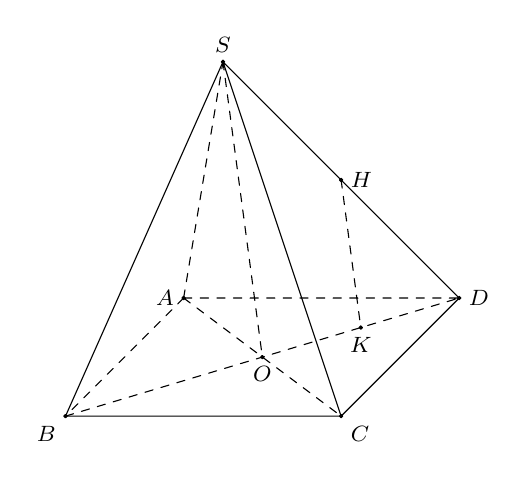
\begin{tikzpicture}[scale=0.5, font=\footnotesize, line join=round, line cap=round, >=stealth]
	\draw[fill=black] (0,0) node[left]{$A$} coordinate (A) circle(1.2pt);
	\draw[fill=black] (-3,-3) node[below left]{$B$} coordinate (B) circle(1.2pt);
	\draw[fill=black] (4,-3) node[below right]{$C$} coordinate (C) circle(1.2pt);
	\draw[fill=black] (7,0) node[right]{$D$} coordinate (D) circle(1.2pt);
	\draw[fill=black] (2,-1.5) node[below]{$O$} coordinate (O) circle(1.2pt);
	\draw[fill=black] (1,6) node[above]{$S$} coordinate (S) circle(1.2pt);
	\draw[fill=black] (4,3) node[right]{$H$} coordinate (H) circle(1.2pt);
	\draw[fill=black] (4.5, -0.75) node[below]{$K$} coordinate (K) circle(1.2pt);
	\draw[dashed] (A)--(S) (A)--(B) (A)--(C) (A)--(D) (B)--(D) (H)--(K) (S)--(O);
	\draw (S)--(B) (S)--(C) (S)--(D) (B)--(C)--(D);
	\end{tikzpicture}}
	}
\end{ex}

\begin{ex}[\textit{Trích đề thi HKI - trường THPT Chuyên Hùng Vương - Năm học 2024-2025}]%[1H4V2-5]
	Cho hình chóp $S.ABCD$ có đáy là hình bình hành tâm $O$, $SAB$ là tam giác đều có độ dài cạnh bằng $4$. Gọi $M$, $N$ theo thứ tự là trung điểm $SC$, $SD$. Hình tạo bởi các đoạn giao tuyến của $(OMN)$ và các mặt của hình chóp có diện tích $S$. Tính $S^2$.
	\par\shortans{$27$}
	\loigiai{
	\begin{center}
	\begin{tikzpicture}[>=stealth,line join=round,line cap=round, font=\footnotesize, scale=.6]
	\path
	(0,0) coordinate (A)
	(7,0) coordinate (B)
	(10,2) coordinate (C)
	(3,2) coordinate (D)
	(4,8) coordinate (S)
	($(S)!1/2!(C)$) coordinate (M)
	($(S)!1/2!(D)$) coordinate (N)
	($(A)!1/2!(D)$) coordinate (P)
	($(B)!1/2!(C)$) coordinate (Q)
	($(A)!1/2!(C)$) coordinate (O)
	;
	\draw (A)--(B)--(C)--(S)--(A) (S)--(B) (M)--(Q);
	\draw[dashed] (A)--(D)--(C) (S)--(D)--(B) (A)--(C) (O)--(M)--(N)--cycle (N)--(P)--(Q);
	\foreach \x/\g in {A/-120,B/-60,C/0,D/130,S/90,M/20,O/-90,N/45,P/90,Q/0}\fill (\x) circle (1pt)+(\g:5mm) node{$\x$};
	\end{tikzpicture}
	\end{center}
	Vì $(OMN)$ có $MN$ song song với $CD$ nên $(OMN)$ cắt $(ABCD)$ theo giao tuyến $PQ$ đi qua $O$ và song song với $MN$, với $P\in AD$, $Q\in BC$.
	\begin{itemize}
		\item $(OMN)$ cắt $(SDC)$ theo giao tuyến $MN$.
		\item $(OMN)$ cắt $(SAD)$ theo giao tuyến $NP$.
		\item $(OMN)$ cắt $(SBC)$ theo giao tuyến $MQ$.
	\end{itemize}
	Suy ra hình tạo bởi các đoạn giao tuyến của $(OMN)$ và các mặt của hình chóp là hình thang $MNPQ$ có hai đáy là $MN$ và $PQ$.\\
	Xét tam giác $ADC$ ta có $O$ là trung đường của $AC$ và $PO\parallel DC$. Suy ra $P$ là trung điểm $AD$.\\
	Suy ra $NP\parallel SA$.\\
	Ta có $NP$, $NO$, $PO$ lần lượt là đường trung bình của các tam giác $SAD$, $SDB$, $ADC$.\\
	Suy ra $NP=\dfrac{1}{2}SA=2$, $NO=\dfrac{1}{2}SB=2$, $PO=\dfrac{1}{2}CD=\dfrac{1}{2}AB=2$, $MN=\dfrac{1}{2}CD=2$, $PQ=AB=4$.\\
	Suy ra các tam giác $ONP$, $OMQ$ và $MNO$ là các tam giác đều bằng nhau và có cạnh bằng $2$.\\
	Ta có $S_{\triangle ONP}=\dfrac{2^2\sqrt3}{4}=\sqrt3$.\\
	Khi này diện tích hình thang $MNPQ$ là
	$$S=3S_{\triangle ONP}=3\sqrt{3}.$$
	Ta có $S^2=\left(3\sqrt{3}\right)^2=27$.
	}
\end{ex}

\Closesolutionfile{ans}

\ind{PHẦN IV.} \inden{Tự luận.}
\setcounter{ex}{0}
\begin{ex}[\textit{Trích SBT Cánh Diều}]%[1H4H2-2]
	Cho tứ diện $ABCD$. Gọi $M$, $N$ lần lượt là trung điểm của $AB$, $AD$ và $P$. là một điểm nằm trên $CD$. Đường thẳng $BC$ cắt mặt phẳng $(MNP)$ tại $Q$. Chứng minh $PQ\parallel BD$.
	\loigiai{
	\immini
	{Vì $BC$ cắt mặt phẳng $(MNP)$ tại $Q$ nên $PQ$ là giao tuyến của $(MNP)$ và $(BCD)$.\\
	Ba mặt phẳng $(ABD)$, $(BCD)$, $(MNP)$ đôi một cắt nhau theo các giao tuyến $BD$, $PQ$, $MN$.\\
	Mà trong tam giác $ABD$, vì $MN$ là đường trung bình nên $MN\parallel BD$.\\
	Vậy theo định lí về giao tuyến của ba mặt phẳng ta có $PQ\parallel BD$.}
	{\begin{tikzpicture}[font=\footnotesize, line join=round, line cap=round, >=stealth, scale=1]
	\path (0,0) coordinate (B) (3.5,0) coordinate (D) (-30:2) coordinate (C) (1,2) coordinate (A)
	($(A)!1/2!(B)$) coordinate (M) ($(A)!1/2!(D)$) coordinate (N) ($(C)!1/3!(D)$) coordinate (P) ($(C)!1/3!(B)$) coordinate (Q);
	\draw (A)--(B)--(C)--(D)--cycle (A)--(C) (N)--(P);
	\draw[dashed] (B)--(D) (N)--(M)--(P)--(Q);
	\foreach \x/\g in {A/90, B/180, D/0, C/-90, M/135, N/45, Q/-135, P/-45}{\fill (\x) circle (1pt)+(\g:0.3)node{$\x$};}
	\end{tikzpicture}}
	}
\end{ex}

\begin{ex}[\textit{Trích SBT Cánh Diều}]%[1H4H2-2]
	Cho hình chóp tứ giác $S.ABCD$. Gọi $G$, $K$ lần lượt là trọng tâm của của các tam giác $SAB$ và $SAD$; $M$, $N$ lần lượt là trung điểm của $BC$ và $CD$. Chứng minh rằng $GK\parallel MN$.
	\loigiai{
	\immini
	{Gọi $P$, $Q$lần lượt là trung điểm của $AB$ và $AD$. Khi đó ta có $\dfrac{SG}{SP}=\dfrac{SK}{SQ}=\dfrac{2}{3}$, suy ra $GK\parallel PQ$.\\
	Vì $PQ$ là đường trung bình của tam giác $ABD$ nên $PQ\parallel BD$; $MN$ là đường trung bình của tam giác $BCD$ nên $MN\parallel BD$. Suy ra $MN\parallel PQ$.\\
	Từ đó suy ra $GK\parallel MN$.}
	{\begin{tikzpicture}[font=\footnotesize, line join=round, line cap=round, >=stealth, scale=1]
	\path (0,0) coordinate (A) (4,0) coordinate (D) (-150:2) coordinate (B) (-50:2) coordinate (C) (-0.5,2) coordinate (S);
	\foreach \x/\y/\z in {A/B/P, B/C/M, C/D/N, D/A/Q}{\path ($(\x)!1/2!(\y)$) coordinate (\z);}
	\path ($(S)!2/3!(P)$) coordinate (G) ($(S)!2/3!(Q)$) coordinate (K);
	\draw (S)--(B)--(C)--(D)--cycle (S)--(C);
	\draw[dashed] (B)--(A)--(D) (S)--(A) (S)--(P)--(Q)--cycle (M)--(N) (B)--(D) (G)--(K);
	\foreach \x/\g in {S/90, A/135, B/-135, C/-90, D/45, M/-135, N/-45, G/135, K/45, P/180, Q/45}{\fill (\x) circle (1pt)+(\g:0.3)node{$\x$};}
	\end{tikzpicture}}
	}
\end{ex}

\begin{ex}[\textit{Trích SBT Kết nối tri thức}]%[1H4H2-4]
	Cho hai hình bình hành $ABCD$ và $ABEF$ không cùng nằm trong một mặt phẳng. Gọi $G$, $H$ lần lượt là giao điểm của hai đường chéo của hai hình bình hành đó. Chứng minh các đường thẳng $GH$, $CE$, $DF$ đôi một song song.
	\loigiai{
	\immini
	{Xét $\triangle AEC$ ta có $\dfrac{AH}{AE}=\dfrac{AG}{AC}=\dfrac{1}{2}$. Theo định lý Thalès đảo suy ra $GH\parallel EC$.\\
	Xét $\triangle BFD$ ta có $\dfrac{BH}{BF}=\dfrac{BG}{BD}=\dfrac{1}{2}$. Theo định lý Thalès đảo suy ra $GH\parallel FD$.\\
	Suy ra $CE\parallel DF$.\\
	Vậy các đường thẳng $GH$, $CE$, $DF$ đôi một song song.}
	{\begin{tikzpicture}[font=\footnotesize, line join=round, line cap=round, >=stealth, scale=1]
	\path (0,0) coordinate (A) (-140:2) coordinate (D) (110:2) coordinate (F)
	(3,0) coordinate (B)+(-140:2) coordinate (C)+(110:2) coordinate (E)
	($(A)!1/2!(C)$) coordinate (G) ($(A)!1/2!(E)$) coordinate (H);
	\draw (E)--(F)--(D)--(C) (E)--(B)--(C)--cycle;
	\draw[dashed] (A)--(B) (F)--(A)--(D) (F)--(B)--(D) (E)--(A)--(C) (G)--(H);
	\foreach \x/\g in {A/180, B/0, D/-135, C/-45, E/45, F/135, G/-90, H/90}{\fill (\x) circle (1pt)+(\g:0.3)node{$\x$};}
	\end{tikzpicture}}
	}
\end{ex}

\begin{ex}[\textit{Trích SBT Kết nối tri thức}]%[1H4H1-3]
	Cho hình chóp $S.ABCD$ có đáy $ABCD$ là hình thang ($AB \parallel CD$). Gọi $M$, $N$ lần lượt là các điểm thuộc các cạnh $SA$, $SD$. Gọi $d$ là giao tuyến của hai mặt phẳng $(MCD)$ và $(NAB)$. Chứng minh rằng $d \parallel AB$.
	\loigiai{
	\immini
	{Gọi $P=AN\cap MD$, khi đó $P\in(MCD)\cap(NAB)$.\\
	Ta có $\heva{&CD\subset(MCD)\\&AB\subset(NAB)\\&CD\parallel AB.}$\\
	Suy ra giao tuyến của $(MCD)$ và $(NAB)$ là đường thẳng $d$ đi qua điểm $P$ và $d\parallel AB \parallel CD$.\\
	Vậy $d\parallel AB$.}
	{\begin{tikzpicture}[font=\footnotesize, line join=round, line cap=round, >=stealth, scale=1]
	\path (0,0) coordinate (A) (-20:2.5) coordinate (D)+(0:1) coordinate (C) (4,0) coordinate (B) (1,3) coordinate (S)
	($(S)!1/2!(A)$) coordinate (M) ($(S)!1/3!(D)$) coordinate (N)
	(intersection of M--D and N--A) coordinate (P);
	\draw (S)--(B)--(C)--(D)--(A)--cycle (D)--(S)--(C) (M)--(D) (N)--(A) (P)--+(180:1.5)node[above]{$d$};
	\draw[dashed] (A)--(B) (M)--(C) (N)--(B) (P)--+(0:1);
	\foreach \x/\g in {S/90, A/135, B/45, C/-45, D/-135, M/135, N/45, P/-90}{\fill (\x) circle (1pt)+(\g:0.3)node{$\x$};}
	\end{tikzpicture}}
	}
\end{ex}

\begin{ex}[\textit{Trích đề thi GKI - trường THPT Dân tộc nội trú - Năm học 2023-2024}]%[1H4H2-3]
	Cho hình chóp $S.ABCD$ có đáy $ABCD$ là hình bình hành. Gọi $M$, $N$ lần lượt là trung điểm của $AD$ và $BC$. Tìm giao tuyến của hai mặt phẳng $(SMN)$ và $(SAB)$.
	\loigiai{
	\immini
	{Ta có $MN$ là đường trung bình của hình bình hành $ABCD$ nên $MN\parallel AB$.\\
	Ta có $S\in(SMN)\cap(SAB)$.\\
	Ta có $\heva{&MN\subset(SMN)\\&AB\subset(SAB)\\&MN\parallel AB.}$\\
	Suy ra $ (SAB)\cap(SMN)=\Delta \parallel AB\parallel MN$ ($\Delta$ đi qua $S$).}
	{\begin{tikzpicture}[line join=round, line cap=round,scale=0.7]
	\coordinate (A) at (0,0);
	\coordinate (B) at (2,-2);
	\coordinate (D) at (5,0);
	\coordinate (C) at ($(B)+(D)-(A)$);
	\coordinate (O) at ($(A)!0.5!(C)$);
	\coordinate (S) at ($(O)+(-1,6)$);
	\coordinate (M) at ($(A)!0.5!(D)$);
	\coordinate (N) at ($(B)!0.5!(C)$);
	\coordinate (P) at ($(S)+(A)-(B)$);
	\coordinate (Q) at ($(S)!-0.5!(P)$);
	\draw (N)--(S)--(A) (S)--(B) (S)--(C) (A)--(B) (B)--(C)(P)--(Q);
	\draw[dashed](A)--(D) (C)--(D) (S)--(D)(S)--(M)--(N);
	\node[above] at (P){$\Delta$};
	\foreach \i/\g in {S/90,A/180,B/-90,C/-90,D/0,M/60,N/-90}{\fill (\i) circle (1pt) ($(\i)+(\g:3mm)$) node[scale=0.7]{$\i$};}
	\end{tikzpicture}}
	}
\end{ex}

\begin{ex}[\textit{Trích đề thi GKI - trường THPT Chuyên Trần Phú - Năm học 2023-2024}]%[1H4H2-2]
	Cho tứ diện $ABCD$. Trên các cạnh $AB$, $AD$ lần lượt lấy các điểm $M$ và $N$ sao cho $\dfrac{AM}{AB}=\dfrac{AN}{AD}=\dfrac{1}{3}$. Gọi $P$, $Q$ lần lượt là trung điểm các cạnh $CD$, $CB$. Chứng minh rằng $MNPQ$ là hình thang.
	\loigiai{
	\immini
	{Xét $\triangle ABD$ có $\dfrac{AM}{AB}=\dfrac{AN}{AD}$ nên $MN \parallel BD$ (định lí Thales đảo).\quad$(1)$\\[0.2cm]
	Xét $\triangle BCD$ có $\dfrac{CQ}{CB}=\dfrac{CP}{CD}=\dfrac{1}{2}$ nên $QP \parallel BD$ (định lí Thales đảo).\quad$(2)$\\[0.2cm]
	Từ $(1)$ và $(2)$ suy ra $MN \parallel PQ$. }
	{\begin{tikzpicture}[scale=1, font=\footnotesize, line join=round, line cap=round, >=stealth]
	%% Khai bao diem
	\path
	(0,0) coordinate (B)
	(5,0) coordinate (C)
	(3.75,-1.5) coordinate (D)
	(2,3.5) coordinate (A)
	($(A)!1/3!(B)$) coordinate (M)
	($(A)!1/3!(D)$) coordinate (N)
	($(C)!1/2!(D)$) coordinate (P)
	($(C)!1/2!(B)$) coordinate (Q)
	;

	\draw (A)--(B)--(D)--(C)--(A)--(D) (M)--(N) (P)--(N);
	\draw[dashed] (B)--(C) (P)--(Q) (M)--(Q);
	%% vẽ điểm
	\foreach \x/\g in {A/90,B/180,C/0,D/-90,M/150,N/50,P/-60,Q/-120}
	\draw[fill=black] (\x) circle (1pt)+(\g:.35)
	node{$\x$};

	\end{tikzpicture}}
	}
\end{ex}

\begin{ex}[\textit{Trích đề thi GKI - trường THPT Chuyên Vị Thanh - Năm học 2023-2024}]%[1H4H2-5]
	Cho hình chóp $S.ABCD$ có đáy là hình thang với các cạnh đáy là $AB$ và $CD$. Gọi $I$, $J$ lần lượt là trung điểm của $AD$ và $BC$. Gọi $G$ là trọng tâm của tam giác $SAB$. Xác định giao tuyến của $(SAB)$ và $(IJG)$.
	\loigiai{
	\immini
	{Do $I$, $J$ lần lượt là trung điểm của $AD$ và $BC$ nên $IJ$ là đường trung bình của hình thang $ABCD\Rightarrow IJ\parallel AB\parallel CD$.\\
	Gọi $d=(SAB) \cap(IJG)$.\\
	Ta có $G$ là điểm chung giữa hai mặt phẳng $(SAB)$ và $(IJG)$.\\
	Mặt khác $\heva{&AB\parallel IJ\\&AB\subset (SAB)\\&IJ\subset (IJG).}$\\
	Suy ra giao tuyến $d$ của $(SAB)$ và $(IJG)$ là đường thẳng qua $G$ và song song với $AB$ và $IJ$.}
	{\begin{tikzpicture}[font=\footnotesize,line join=round, line cap=round, >=stealth,scale=1]
	\foreach \x/\y/\pos in {0/0/A, -1.25/-1.5/D, 5/0/B} \path ($(\x,\y)$) coordinate (\pos);
	\path 
	($(D)+(3,0)$) coordinate (C)
	($(A)!1/2!(D)$) coordinate (I)
	($(C)!.5!(B)$)coordinate(J)
	($(A)!.5!(B)$)coordinate(M)
	($(A)+(1,3)$) coordinate (S)
	($(S)!2/3!(M)$)coordinate(G)
	;
	\draw[dashed] (B)--(A)--(D) (M)--(S)--(A)
	(I)--(J)--(G)--cycle
	;
	\draw (C)--(S)--(B)--(C)--(D)--(S);
	\foreach \x/\pos in {S/90, A/180, B/0, C/-90, D/-90, G/45,I/-90,J/-90} \fill (\x) circle(1pt) node[{shift=(\pos:0.25)}]{$\x$};
	\end{tikzpicture}}
	}
\end{ex}

\begin{ex}[\textit{Trích đề thi GKI - trường THPT Hoàng Long - Năm học 2023-2024}]%[1H4V2-2]
	Cho tứ diện $ABCD$. Gọi $I$, $J$ lần lượt là trọng tâm tam giác $ABC$, $ABD$. Hai đường thẳng $IJ$ và $CD$ có vị trí tương đối gì và tỉ số $\dfrac{IJ}{CD}$ bằng bao nhiêu?
	\loigiai{
	\immini
	{Gọi $M$, $N$ lần lượt là trung điểm của $BC$ và $BD$.\\
	Ta có 
	$\heva{&MN=\dfrac{1}{2}CD\\& MN\parallel CD}$ 
	(vì $MN$ là đường trung bình $\triangle{BCD}$).\\
	Mặt khác $\dfrac{AI}{AM}=\dfrac{AJ}{AN}=\dfrac{2}{3}\Rightarrow \heva{&IJ=\dfrac{2}{3}MN\\& IJ\parallel MN.}$\\
	Vậy $IJ\parallel CD$ và $IJ=\dfrac{1}{3}C$.}
	{\begin{tikzpicture}[>=stealth,line join=round,line cap=round,font=\footnotesize,scale=0.75]
	\coordinate (B) at (-2,1);
	\coordinate (A) at (0,6);
	\coordinate (C) at (3.5,-2);
	\coordinate (D) at (6.5,2);
	%\coordinate (S) at ($(A)+(100:3)$);
	\coordinate (N) at ($(B)!1/2!(D)$);
	\coordinate (M) at ($(C)!1/2!(B)$);
	\coordinate (I) at ($(A)!2/3!(M)$);
	\coordinate (J) at ($(A)!2/3!(N)$);
	\draw (C)--(A) node[left]{$A$}--(B) node[above left]{$B$}--(C) node[below left]{$C$}--(D) node[below right]{$D$}--(A);
	\draw (A)--(I);
	\draw[dashed] (B)--(D);
	\draw (I) node[left]{$I$}--(M) node[below left]{$M$};
	\draw[dashed] (N) node[above right]{$N$}--(J) node[above right]{$J$}--(A);
	\draw[dashed] (I)--(J) (N)--(M);
	\foreach \diem in {A,B,C,D,M,N,I,J}
	\fill (\diem)circle(1pt);
	\end{tikzpicture}}
	}
\end{ex}

\begin{ex}[\textit{Trích đề thi GKI - trường THPT Nguyễn Trãi - Năm học 2023-2024}]%[1H4H2-5]
	Cho hình chóp $S.ABCD$, đáy $ABCD$ là hình thang có $AB\parallel CD$ và $AB=3CD$. Trên cạnh $SB$ lấy điểm $M$ sao cho $SM=\dfrac{1}{3}SB$.
	\begin{enumerate}
		\item Xác định giao điểm $N$ của đường thẳng $SC$ và mặt phẳng $(ADM)$. Tính tỉ số $\dfrac{SC}{SN}$.
		\item Gọi $I$, $J$ lần lượt là trung điểm của các cạnh $AD$, $BC$ và $G$ là trọng tâm tam giác $SAB$. Mặt phẳng $(IJG)$ cắt $SA$, $SB$ lần lượt tại $E$ và $F$. Chứng minh tứ giác $IEFJ$ là hình bình hành.
	\end{enumerate}
	\loigiai{
	\begin{center}
	\begin{tikzpicture}[>=stealth,line join=round,line cap=round]
	\path (-0.5,4) coordinate (S)
	(0,0) coordinate (A) (6,0) coordinate (B) (-150:3) coordinate (D)+(2,0) coordinate (C)
	($(S)!1/3!(B)$) coordinate (M)
	(intersection of A--D and B--C) coordinate (H)
	(intersection of H--M and S--C) coordinate (N)
	($(M)!1/3!(B)$) coordinate (K)
	($(A)!1/2!(D)$) coordinate (I) ($(B)!1/2!(C)$) coordinate (J)
	(barycentric cs:S=1,A=1,B=1) coordinate (G)
	($(A)!1/2!(B)$) coordinate (P)
	($(S)!2/3!(A)$) coordinate (E) ($(S)!2/3!(B)$) coordinate (F);
	\draw (K)--(C)--(S)--(H)--(B)--(S) (H)--(M) (F)--(J);
	\draw[dashed] (H)--(S)--(A)--(H) (B)--(A)--(M)--(D)--(C) (S)--(P) (I)--(G)--(J)--(I)--(E)--(F);
	\foreach \diem/\g in {A/135 ,B/0, C/-45, D/-45, S/90, I/-45, J/-45, M/45, N/135, H/-135, G/45, K/45, P/-135, E/135, F/45}{\fill[black](\diem)circle(1pt)+(\g:0.3)node{$\diem$};}
	\end{tikzpicture}
	\end{center}
	\begin{enumerate}
		\item Trong mặt phẳng $(ABCD)$, gọi $H$ là giao điểm của $AD$ và $CB$.\\
		Nối $H$ với $M$, $HM$ cắt $SC$ tại $N$.\\
		Khi đó $N$ là giao điểm của $(ADM)$ và $SC$.\\
		Vẽ $CK\parallel HM$, từ giả thiết ta có\\
		$\dfrac{DC}{AB}=\dfrac{HC}{HB}=\dfrac{MK}{MB}=\dfrac{1}{3}\Rightarrow MK=\dfrac{1}{3}MB=\dfrac{1}{3}\cdot 2SM=\dfrac{2}{3}SM$.\\
		Mà $\dfrac{SC}{SN}=\dfrac{SK}{SM}=\dfrac{SM+MK}{SM}=1+\dfrac{MK}{SM}=1+\dfrac{2}{3}=\dfrac{5}{3}$.\\
		Vậy $\dfrac{SC}{SN}=\dfrac{5}{3}$.
		\item Ta có $IJ\parallel AB$ vì $IJ$ là đường trung bình của hình thang $ABCD$ và\\
		$(IJG)\cap(SAB)=\{G\}$\\
		$(IJG)\cap(SAB)=Gx\parallel AB\parallel IJ$.\\
		Gọi $E=Gx\cap SA$, $F=Gx\cap SB$ suy ra $AB\parallel IJ\parallel EF$, tứ giác $IJFE$ là hình thang.\\
		Mặt khác, $G$ là trọng tâm tam giác $SAB$ suy ra $SG=\dfrac{2}{3}GP$ với $P$ là trung điểm của $AB$.\\
		$\Rightarrow EF=\dfrac{2}{3}AB=\dfrac{2}{3} \cdot 3CD=2CD$. \quad $(1)$\\
		$IJ$ là đường trung bình của hình thang $ABCD$ nên $IJ=\dfrac{AB+CD}{2}=2CD$. \quad $(2)$\\
		Từ $(1)$ và $(2)$ suy ra $IJ=EF$.\\
		Vậy tứ giác $IEFJ$ là hình bình hành.
	\end{enumerate}
	}
\end{ex}

\begin{ex}[\textit{Trích đề thi GKI - trường THPT Nguyễn Hữu Tiến - Năm học 2023-2024}]%[1H4C2-5]
	Cho hình chóp $S.ABCD$ có đáy $ABCD$ là hình bình hành tâm $O$. Gọi $M$, $N$, $P$ lần lượt là trung điểm của $SB$, $SD$ và $OC$.
	\begin{enumerate}
		\item Tìm giao tuyến của $(SBD)$ và $(SAC)$.
		\item Tìm giao tuyến của $(MNP)$ và $(SAC)$.
		\item Tìm giao điểm của $SA$ và $(MNP)$.
		\item Xác định thiết diện của hình chóp $S.ABCD$ cắt bởi $(MNP)$.
	\end{enumerate}
	\loigiai
	{ 
	\begin{center}
	\begin{tikzpicture}[scale=1, font=\footnotesize, line join=round, line cap=round, >=stealth]
	\path (0,0) coordinate (A) (6,0) coordinate (D) (-155:4) coordinate (B)+(6,0) coordinate (C)
	(80:5) coordinate (S);
	\foreach \a/\b/\c in {A/C/O, S/B/M, S/D/N, O/C/P, C/B/Q, C/D/R}{\path ($(\a)!1/2!(\b)$) coordinate (\c);}
	\path (intersection of M--N and S--O) coordinate (K)
	(intersection of P--K and S--A) coordinate (H);
	\draw (B)--(C)--(D)--(S)--cycle (S)--(C) (Q)--(M) (N)--(R);
	\draw[dashed] (C)--(A)--(D)--(B) (O)--(S)--(A)--(B) (M)--(N)--(P)--cycle (K)--(P)--(H) (R)--(Q) (M)--(H)--(N);
	\foreach \diem/\g in {A/135, B/-135, C/-45, D/45, S/90, O/-90, M/135, N/45, P/-90, K/-135, H/135, R/-45, Q/-90}{\fill (\diem)circle(1pt)+(\g:0.25)node{$\diem$};}
	\end{tikzpicture}
	\end{center}

	\begin{enumerate}
		\item Ta có $\heva{& O \in AC, AC \subset (SAC) \\ & O \in BD, BD \subset (SBD) }\Rightarrow O \in (SBD) \cap (SAC)$.\\
		Và $S \in (SBD) \cap (SAC)$.\\
		Suy ra $SO=(SBD) \cap (SAC)$.
		\item Trong $(SBD)$, gọi $K=MN\cap SO$.\\
		Ta có $\heva{& K \in SO, SO \subset (SAC) \\ & K \in MN, MN \subset (MNP) }\Rightarrow K \in (MNP) \cap (SAC)$.\quad $(1)$\\
		Ngoài ra $P \in (MNP) \cap (SAC)$. \quad $(2)$\\
		Từ $(1)$ và $(2)$ suy ra $KP = (MNP) \cap (SAC)$.
		\item Trong $(SAC)$, gọi $H=PK \cap SA$.\\
		Ta có $\heva{& H \in SA \\ & H \in PK, PK \subset (MNP) }\Rightarrow H =SA \cap (MNP)$.
		\item Ta có $\heva{& P \in (MNP) \cap (ABCD) \\ & MN \subset (MNP), BD \subset (ABCD)\\ & MN \parallel BD.}\\
		\Rightarrow Px = (MNP)\cap (ABCD)$ với $Px\parallel BD\parallel MN$.\\
		Trong $(ABCD)$, gọi $Q = Px \cap BC$, $R=Px \cap DC$.\\
		Ta có $\heva{& (MNP)\cap (SAB)=MH \\ & (MNP)\cap (SAD)=HN\\& (MNP)\cap (SDC)=NR\\& (MNP)\cap (ABCD)=RQ\\& (MNP)\cap (SBC)=QM.}$\\
		Suy ra thiết diện của hình chóp $S.ABCD$ cắt bởi $(MNP)$ là ngũ giác $MHNRQ$.
	\end{enumerate} 
	}
\end{ex}
